% !TEX root = ../my-thesis.tex
%
\chapter{Introduction}
\label{sec:intro}

\cleanchapterquote{
	\textgreek{Δέδυκε μὲν ἀ σελάννα}\\
	\textsuperscript{The moon and the Pleiades}\\
	\textgreek{καὶ Πληΐαδες, μέσαι δέ}\\
	\textsuperscript{have set, it is}\\
	\textgreek{νύκτες, πάρα δ' ἔρχετ' ὤρα,}\\
	\textsuperscript{midnight, time is passing,}\\
	\textgreek{ἔγω δὲ μόνα κατεύδω.}\\
	\textsuperscript{but I sleep alone.}\\
}{Sappho, `The Midnight Poem'}{(c. 600 BC)}

% ---------------------------------------
\section{From seven sisters to a powerhouse of astronomy}
\label{sec:intro:intro}

In all of astronomy, few objects have retained relevance throughout the centuries as much as open clusters (OCs). Easily visible to the naked eye, the Pleiades has been observed since at least the dawn of civilisation \citep{rappengluck_palaeolithic_timekeepers_2001,mozel_sky_disk_2003}, along with a handful of other OCs visible without a telescope. In the present day, the now thousands of known OCs are a key tool in modern astronomy for understanding stellar and galactic evolution.

% TODO: this paragraph annoys me
Star clusters are formed when clouds of cold molecular gas collapse due to gravity, forming stars. Sometimes, when star formation occurs densely enough, these stars fall further into gravitationally bound clusters that can survive in the galactic disk for as long as $\sim 10^9$~years \citep{lada_embedded_2003,portegies_zwart_young_2010}. It is this property of the formation of OCs that makes them so useful: having formed at the same time and from the same molecular cloud, all stars in an OC will have the same age and initial chemical composition, and will remain co-located in space in a dense cluster. Even hundreds of millions of years after an OC forms, the parameters of the cluster's member stars can be measured significantly more precisely than when studying stars in isolation. 

For instance, when a parameter such as the distance of member stars can simply be averaged over all member stars, then the precision of the mean distance of an OC (and hence the distance to all of its member stars) will be a factor $\sqrt{n}$ more precise than the distance to any individual star. Alternatively, when a property such as chemical composition is highly time consuming to derive, it can be derived for a fraction of stars in an OC and be applied relatively safely to all stars in a cluster.

The ease of studying stellar astrophysics with OCs results in OCs having an extremely wide range of scientific use cases. For instance, OCs are used as testing grounds for stellar evolution models \citep{bressan_parsec_2012}, as tracers of galactic structure \citep{cantat-gaudin_painting_2020,castro-ginard_milky_2021}, or even as calibrators of Cepheid variable stars \citep{medina_revisited_2021}, which are an essential first rung on the cosmic distance ladder and are vital in the derivation of the cosmological parameters of the universe. It is somewhat of a cliché to describe OCs as `the laboratories of stellar evolution', but it really is true: OCs are a fantastic way to observe stars of a given age and composition across a broad range of masses, and to do so with orders of magnitude more precision than when studying isolated field stars.

The best part of the modern story of the OC's contribution to astrophysics comes with the \gaia\ satellite, however. In just five years since its first full data release \citep{brown_gaia_2018}, \gaia\ has revolutionised the study of our galaxy, including the study of OCs; with dozens of papers reporting thousands of new objects \citep[e.g.][]{liu_catalog_2019,castro-ginard_hunting_2019,castro-ginard_hunting_2020,castro-ginard_hunting_2022}, and a number of works deriving dramatically improved parameters and members for OCs in the Milky Way \citep[e.g.][]{cantat-gaudin_gaia_2018,tarricq_3d_2020}. Arguably, there has never been a better time to do science with OCs, owing to the incredible quantity and quality of data that \gaia\ has provided.

There is, however, a catch. Even though the Milky Way is estimated to contain as many as $10^5$ OCs \citep{dias_new_2002}, there are still only a few thousand currently known in the literature -- representing a small fraction of the total number of OCs in our galaxy. It has been shown that the census of OCs is incomplete within even 1~kpc from the Sun \citep[e.g.][]{castro-ginard_new_2018}, and the extent of the remaining incompleteness is unknown. Worse still, it has been shown that many of the OCs catalogued previously in the literature may not exist \citep{cantat-gaudin_clusters_2020,piatti_catching_2023}, with it being largely unknown which OCs are or are not real. The many fantastic uses of OCs in other areas of astronomy are contingent on a reliable, accurate, and complete census of OCs; and the many current caveats with the census of OCs limit the science potential of these fantastic objects, in a time when we have more available data with which to study them than ever before.

% TODO: this paragraph is too weak
In this thesis, I will present solutions to a number of the current issues with the OC census in the era of \gaia, using a range of data analysis and parameter inference techniques. I will then use these techniques to create the largest census of OCs to date and derive a range of parameters for these OCs. With this thesis, I also hope to present methods that could continue to be used to maximise the quality of the OC census for the coming decade of \gaia\ data releases -- as well as for whatever instruments supercede \gaia\ in the future.

Before launching into the chapters detailing my work over the past three and a half years, it is worth first conducting an overview of the science behind OCs in the introduction to this thesis. In Sect.~\ref{sec:intro:pre-gaia}, I will discuss the history of OC observations up to before the release of \gaia\ DR2 in 2018. Section~\ref{sec:intro:gaia} will then discuss the stunning data of \gaia\ and how it has already thoroughly revolutionised our understanding of OCs in just a handful of years. Section~\ref{sec:intro:aims} reviews the current issues with the OC census and discusses the broad aims of this thesis. Finally, Sect.~\ref{sec:intro:theory} will briefly discuss some key concepts from both observational and theoretical studies of OCs, providing background that will assist with the reading of this thesis.

The nomenclature and definition of star clusters varies throughout the literature. Hence, in the next section, I will discuss a working definition of OCs that I will adopt throughout the rest of this work.


% ---------------------------------------
\section{The definition of an open cluster}
\label{sec:intro:definition}

\begin{figure}[tb]
	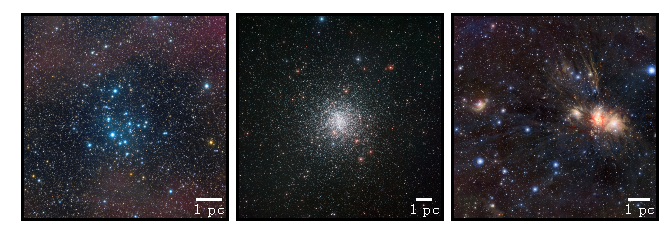
\includegraphics[width=\textwidth]{fig/c1/oc_gc_mg_comparison.pdf}
	\caption[A visual comparison between the three main types of star cluster found in the Milky Way]{A visual comparison between the three main types of star cluster found in the Milky Way. \emph{Left:} the open cluster NGC~2547. \emph{Middle:} the globular cluster M4. \emph{Right:} the moving group/OB association Monoceros~R2. All images contain a scale in the bottom right showing a length of 1~pc at the distance of each cluster. \emph{Credit, left to right:} ESO / J. Pérez; ESO; ESO / J. Emerson / VISTA. }
	\label{fig:intro:definition:comparison}
\end{figure}

There are many different types of star cluster in the universe. Avoiding confusion when talking about star clusters is important, particularly since observers and theorists often use very different nomenclature. Definitions of star clusters can differ significantly even in observational communities when comparing between galactic and extra-galactic astronomy. Hence, before going any further, it is important to define exactly what I will be discussing in this thesis; I will use the following definitions consistently throughout this thesis for clarity.

This thesis will almost exclusively discuss clusters observed in the Milky Way, which are traditionally divided into three broad categories. I will primarily discuss open clusters, although I will also touch on globular clusters and moving groups. I differentiate between these three types of cluster as follows, matching the observational definitions in \cite{portegies_zwart_young_2010}.

\textbf{Open clusters} (OCs) are gravitationally bound clusters with a typical age of around 100~Myr, although some are older than 1~Gyr and some are as young as 0.1~Myr. OCs have masses of typically no greater than $10^4$~\MSun\ and may be made up of a few dozen to a few thousand stars, with a typical minimum being ten stars. OCs are remants of recent star formation, and are hence predominantly located in the galactic disk where the star formation rate is highest. Most OCs have a size of around 3 to 10~pc. Other than some rare, potential exceptions, OCs contain a single population of stars.

\textbf{Globular clusters} (GCs) are much older and more massive gravitationally bound clusters, with ages typically greater than 10~Gyr and masses typically greater than $10^5$~\MSun. The largest GCs can contain a million stars or more. GCs have a typical size of around 10 to 20~pc. GCs tend to reside in the galactic bulge or in the galactic halo. Many GCs contain multiple populations of stars. Almost all OCs have masses significantly lower than the typical present day mass of GCs, although observations of a handful of young massive clusters in the Milky Way such as Westerlund~1 (sometimes also referred to as `super star clusters') as well as observations of galaxies with more active star formation suggest that the highest mass star clusters will be long-lived, and may evolve into GCs. However, this is not the case for almost all OCs that I will study in this thesis, as the only young massive clusters in the Milky Way are generally distant, heavily reddened, and outside of the reach of the visual-band observations of the \gaia\ telescope.

\textbf{Moving groups} (MGs) are of a similar mass and number count to OCs, except they are not gravitationally bound. Due to this, they disperse much more quickly, and hence often have much younger ages. MGs have the widest definition, and encompass any group of stars that are comoving and coeval, but are specifically \emph{not} gravitationally bound. Many MGs are referred to as `OB associations' in the literature, due to them often containing a number of young, high mass O and B stars. 

\begin{table}[tb]
	\caption{Approximate definitions for the three types of star cluster that will be discussed in this thesis.\label{tab:intro:definition:definition}}
	\begin{tabularx}{\textwidth}{l | X | X | X | X}
		\hline\hline
		Type & Bound? & Age & Mass & Location \\
		\hline
		Open cluster (OC)   & Weakly & $\lesssim 1$ Gyr & $\lesssim 10^4$ \MSun & Disk \\
		Globular cluster (GC)   & Strongly & $\gtrsim 10$ Gyr & $\gtrsim 10^5$ \MSun & Halo/Bulge \\
		Moving group (MG)   & No & $\lesssim 50$ Myr & $\lesssim 10^3$ \MSun & Disk\\
		\hline
	\end{tabularx}
\end{table}

These definitions are summarised in Table~\ref{tab:intro:definition:definition} and compared visually in Fig.~\ref{fig:intro:definition:comparison}. The figure shows three clusters; NGC~2547, M4, and Monoceros~R2. NGC~2547 is a sparser OC that has a clear core of young blue stars at its center, about $\sim 1$~pc across. On the other hand, despite being only slightly larger, the GC M4 clearly contains significantly more stars. The stars in M4 are older, with the cluster having a whiter appearance along with more evolved red giant stars. Finally, the MG Monoceros~R2 is simply a group of young blue stars, with no discernible core. 





% ---------------------------------------
\section{The pre-\gaia\ history of open cluster observations}
\label{sec:intro:pre-gaia}

While the results of this thesis are entirely derived using data from \gaia, to truly understand just how groundbreaking the current data of the \gaia\ satellite is, it is worth first briefly reviewing the history of OC observations.


\subsection{Open clusters up to the 20th century}

% Plot of the pleiades
\begin{figure}[t]
	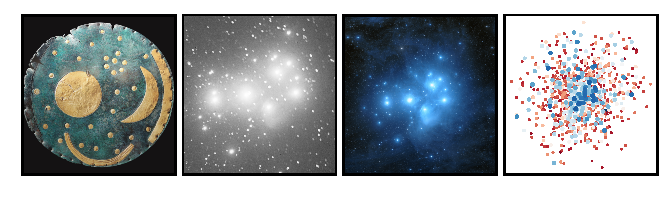
\includegraphics[width=\textwidth]{fig/c1/pleiades.pdf}
	\caption[The Pleiades as depicted throughout history]{The Pleiades, as depicted throughout history and showing the clear improvements in astronomical data gathering over time. \emph{Left:} the Nebra Sky Disc, depicting the Pleiades with its seven naked-eye visible stars in the upper center. The disc was discovered in 1999 in northern Germany and is dated to between 1800-1600 BC. \emph{Middle left:} the Pleiades, as imaged in 1909 with Wolf's Doppelastrograph at the Landessternwarte Heidelberg-Königstuhl. \emph{Middle right:} the Pleiades, as imaged by Hubble. \emph{Right:} the $\sim$1000 member stars for the Pleiades extracted from \gaia\ DR2 data and isolated from field stars by \cite{cantat-gaudin_characterising_2018}. Each star is represented by a point scaled by its magnitude and coloured according to its $BP-RP$ colour. \emph{Credits:} Frank Vincentz; Heidelberg Digitized Astronomical Plates; Davide De Martin \& NASA/ESA Hubble.}
	\label{fig:intro:history:pleiades}
\end{figure}

Our ability to observe OCs has progressed incredibly far throughout the history of astronomy (Fig.~\ref{fig:intro:history:pleiades}). The invention of the refracting telescope allowed for early astronomers such as Galileo to observe that OCs and GCs are in fact clusters of many stars, as opposed to being dispered single sources as previously believed from unaided observations. It was, however, the invention and widespread adoptation of the reflecting telescope in the 17\textsuperscript{th} and 18\textsuperscript{th} centuries that led to catalogues of clusters like we use today.

% Plot of catalogues of OCs
\begin{figure}[tb]
	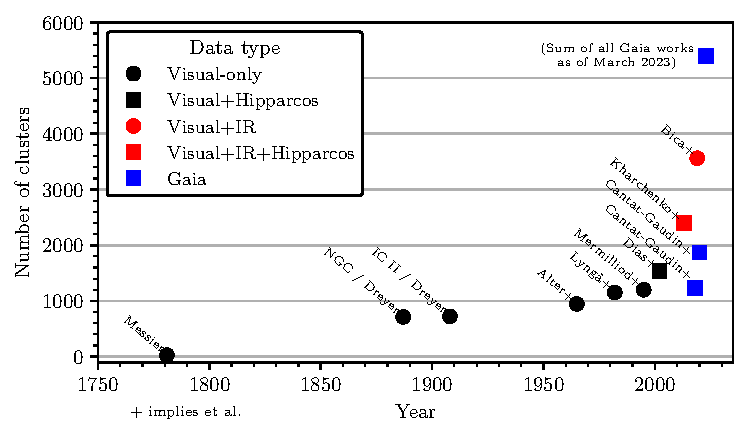
\includegraphics[width=\textwidth]{fig/c1/catalogues.pdf}
	\caption[The size of OC catalogues over time]{The size of OC catalogues over time. After the initial rise in the size of catalogues due to the advent of reflecting telescopes in the 18\third\ and 19\third\ centuries, it was not until the past 25 years and the advent of large-scale astrometric and IR datasets that the OC census significantly increased in size. \\
	{\footnotesize N.B.: this is not an exhaustive plot of all catalogues, and a number of old catalogues such as \cite{herschel_catalogue_one_1786} and \cite{herschel_general_catalogue_1864} without digitised versions are not included.}}
	\label{fig:intro:history:catalogues}
\end{figure}

The power of reflecting telescopes allowed astronomers to scan the sky to signficantly greater depth, searching for clusters of stars and discovering many new objects in the process \citep[e.g.][]{herschel_catalogue_one_1786}, with the number of known OCs jumping from a few dozen to around 700 in a little over a century. Figure~\ref{fig:intro:history:catalogues} shows the evolution in size of OC catalogues over time, showing the rise to around 700 clusters by the turn of the 20\textsuperscript{th} century. Many of the OCs known and catalogued by astronomers at this point were some of the largest and most scientifically useful, with many of these OCs (especially those in the NGC catalogue) being some of the most frequently studied objects even today. 

% Plot of CMDs of OCs
\begin{figure}[tb]
	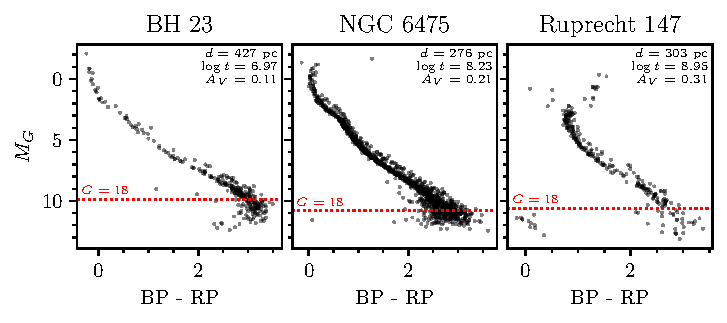
\includegraphics[width=\textwidth]{fig/c1/cmd_comparison.pdf}
	\caption[A comparison of the CMDs of a number of nearby OCs]{A comparison of the CMDs of a number of nearby OCs, using membership lists from later in this thesis in Sect.~\ref{sec:census} and plotted with their absolute magnitude $M_G$ against colour $BP - RP$. The OCs are plotted from left to right in order of increasing age, with their distance $d$, logarithmic age $\log t$ and extinction $A_V$ shown in the top right. The dashed red line indicates the approximate 100\% completeness limit of these OC membership lists, with sources fainter than an apparent magnitude of $G=18$ frequently being missed and often having under-estimated $BP-RP$ colours. BH~23 is less than 10~Myr old and has almost no main sequence turn off; NGC~6475 is over 100~Myr old and has a clear turn off; Ruprecht~147 is around 1~Gyr old and even has a clear population of white dwarf stars.}
	\label{fig:intro:history:cmds}
\end{figure}

The 20\textsuperscript{th} century saw improvements to data gathering and techniques, with early photometric and spectroscopic methods allowing authors such as \cite{rosenberg_uber_zusammenhang_1910} and \cite{hertzsprung_ueber_verwendung_1911} to plot the brightness of the stars in the Pleiades and the Hyades against their spectral features, noticing for the first time that the brightness of stars is related to their colour and spectral features. \cite{russell_relations_spectra_1914} derived the absolute magnitude of stars in the Hyades and ploted this against an early spectral analogue of the temperature of its member stars, plotting the luminosity of stars against their temperature for the first time and inventing `Hertzsprung-Russell' or `colour-magnitude' diagrams (CMDs), a type of plot still used extensively in the present day as an essential tool to understand stellar evolution. Later, the differences in CMDs between different clusters were noticed. This was interpreted as being a difference in age between the clusters, allowing for the ages of stars within star clusters to be estimated, and beginning the foundation of our knowledge of stellar evolution (Fig.~\ref{fig:intro:history:cmds}).

While the 20\textsuperscript{th} century saw huge strides in our understanding of stars and star clusters, the size of OC catalogues went relatively unchanged (Fig.~\ref{fig:intro:history:catalogues}). It was not until the 1990s and the arrival of new methodologies that the OC census itself has begun its largest upheaval since the widespread adoptation of reflecting telescopes more than 200 years prior.


\subsection{The advent of modern astrometry and infra-red datasets}

The launch of the \emph{Hipparcos} satellite and subsequent data releases \citep{perryman_hipparcos_1997} produced a catalogue of around 10$^5$ sources with five-parameter milliarcsecond-precision astrometry. OCs stand out as overdensities in \emph{Hipparcos} data, in particular in proper motions, as OCs are comoving groups of stars that often have different velocities to background field sources. This new data allowed works such as \cite{platais_search_1998} to discover a number of new OCs, with many being small objects near to the Sun that evaded detection with only two-dimensional visual observations. 

The catalogue of \cite{dias_new_2002} included over 300 more objects than the roughly ten years prior catalogue of \cite{mermilliod_database_1995} (Fig.~\ref{fig:intro:history:catalogues}), representing the largest 
major jump in the size of the OC census in over a century, in addition to the much more accurate mean cluster proper motions and parallaxes provided by \emph{Hipparcos}. However, this was just the beginning, and more new science was to come.

Data releases from the Two Micron All Sky Survey \citep[2MASS,][]{skrutskie_two_2006} in the 2000s provided the next major jump in data availability for furthering OC science. The infrared (IR) data of 2MASS and its associated catalogue of 471 million point sources allowed works such as \cite{dutra_new_2001}, \cite{dutra_new_infrared_2003}, \cite{bica_new_infrared_2003}, and \cite{froebrich_systematic_2007} to uncover over a thousand new OC candidates in the galactic disk, using IR data to peer through insterstellar dust and unveil many previously-obscured objects for the first time. In addition, works around this time began to make increasing use of advances in computing power, with works such as \cite{froebrich_systematic_2007} using automated retrieval to extract cluster candidates instead of simply scanning datasets by eye for overdensities.

Work predominantly with IR data culminated in the catalogue of \cite{kharchenko_global_2013}, who derived homoegeneous membership lists, ages, extinctions, distances, proper motions, radii, and many other parameters for a total of 3006 clusters, 2399 of which are OCs or probable OCs, using a combination of 2MASS data and astrometric data from the PPMXL catalogue of proper motions \citep{roeser_ppmxl_catalog_2010}.

In around 20 years, the OC census more than doubled in size between the work of \cite{mermilliod_database_1995} to the work of \cite{kharchenko_global_2013}. This unprecedented shift represented the first time that the OC census had been significantly expanded in over a century, with improved datasets offering significantly better measurements of more clusters than ever before. 

Yet the seismic shift in cluster catalogues brought about by IR datasets and \emph{Hipparcos} was scarcely the beginning of the modern revolution in studies of OCs. \gaia's first full data release in 2018, DR2 \citep{brown_gaia_2018}, sparked the next revolution in the census of OCs.


\section{The \gaia\ revolution}
\label{sec:intro:gaia}

For almost all of the history of astronomy, our view of the Milky Way has been strictly two-dimensional. Observing a three-dimensional galaxy in two dimensions is inherently limiting; it took until the 20\third\ century to even discover that galaxies are separate from the Milky Way \citep{curtis_novae_spiral_1917}. Although astrometric parameters like parallaxes have been measured for stars for over a century, and can be used to view the stars of the galaxy in three dimensions, these datasets have always been limited to a few hundred or thousand stars until very recently. %In addition, while proper motions have long been measured for stars, sometimes even in datasets containing hundreds of millions of sources \citep[e.g.][]{roeser_ppmxl_catalog_2010}, the precision of \gaia's proper motion measurements are orders of magnitude better than even the best ground-based proper motion studies -- allowing for multitudes of exciting new science.


\subsection{Background on the \gaia\ satellite}
\label{sec:intro:history:gaia:background}

\gaia\ is a space-based telescope launched in 2013 that aims to measure a wealth of parameters to an unprecedented level of precision for around $10^9$ stars. \gaia\ is measuring precise positions, proper motions, parallaxes, and photometry for its full sample of stars, and also measures radial velocities and low-resolution spectra for brighter subsamples of sources \citep{gaia_collaboration_gaia_2016}. It is the incredible scale and precision of \gaia\ data that sets it apart from any previous datasets.

% Plot of hipparcos vs. gaia astrometric accuracy
\begin{figure}[tb]
	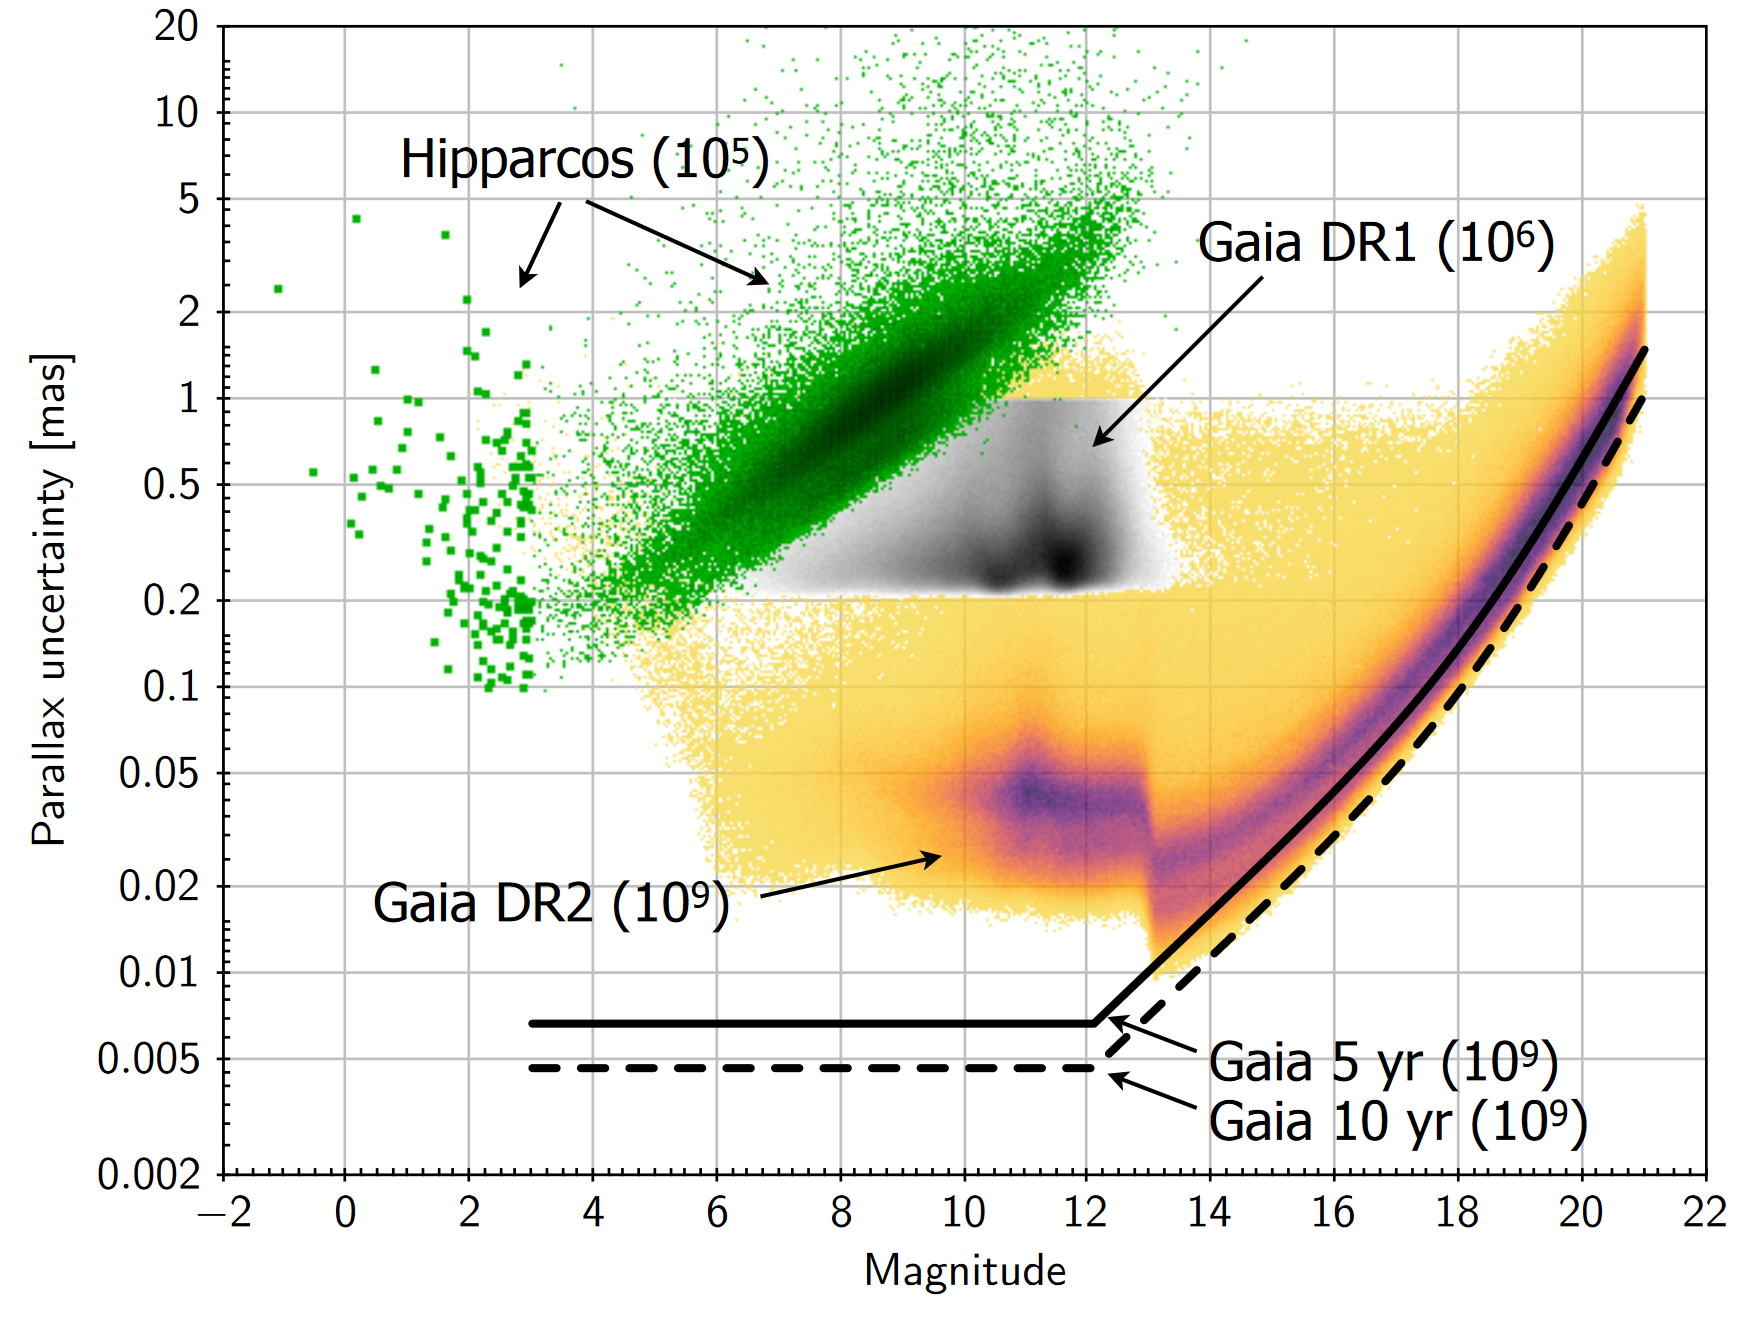
\includegraphics[width=\textwidth]{fig/c1/gaia_dr2_astrometry.png}
	\caption[Comparison between the astrometric accuracy for Hipparcos, Gaia, and future Gaia data releases]{Comparison between the astrometric accuracy for all sources in the final data release of Hipparcos, \gaia\ DR1, and \gaia\ DR2. The predicted accuracy of future data releases using 5 and 10 years of data is shown by the solid and dashed lines respectively. \emph{Credit}: \gaia\ DPAC.}
	\label{fig:intro:history:gaia_accuracy}
\end{figure}

Figure~\ref{fig:intro:history:gaia_accuracy} shows a comparison of the parallax uncertainty of \gaia\ data against data from the \emph{Hipparcos} satellite. The difference in accuracy and quantity of data is clear: \gaia\ can measure parallaxes for $10^4$ times as many stars at a projected eventual accuracy as much as $10^3$ times better than \emph{Hipparcos}. Inevitably, such a large increase in the amount (and quality) of data has huge implications for the study of all objects in the Milky Way, of course including OCs.

% Plot of gaia astrometric tracks
\begin{figure}[tb]
	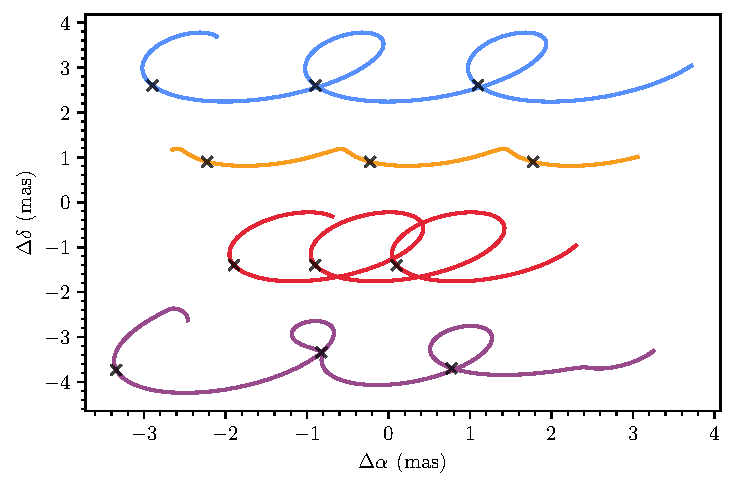
\includegraphics[width=\textwidth]{fig/c1/tracks.pdf}
	\caption[The predicted on-sky astrometric tracks of stars with different parameters]{The predicted on-sky astrometric tracks of stars with different parameters, generated using astromet \citep{penoyre_astrometric_2022}. All sources are at coordinates $\alpha,\,\beta=(0\degree,\,45\degree)$, but are offset in the $y$ direction for clarity of plotting. The first source has $\mu_{\alpha^*}=2$~masyr\textsuperscript{-1}, $\mu_{\delta}=0$, and is at a distance of 1~kpc. In the second example, the distance is quadrupled relative to the first. In the third example, the proper motion is halved relative to the first. In the final example, a binary with a period close to 1~yr, high eccentricity, and a low light ratio is added to the first example, producing a highly irregular track. The crosses denote the position of each source in one-year intervals.}
	\label{fig:intro:history:gaia_tracks}
\end{figure}

To truly understand the wonder of the \gaia\ satellite, it is first worth discussing how exactly it works. Although our galaxy is a dynamic system, with stars continually orbiting around the centre of the Milky Way \citep{binney_galactic_1987}, it is exceptionally difficult to capture the movement of our galaxy in real time. To the human eye, the night sky is static; even the closest stars with the highest proper motions and parallaxes have movements across the sky measured in arcseconds, with one arcsecond being equivalent to just $1/3600$ of a degree. For stars at a distance of, say, 1~kpc, their parallax will amount to just 1~mas. With the Milky Way having an estimated radius of between roughly 15 to 25~kpc \citep{lopez-corredoira_disk_stars_2018}, it is clear that measuring precise astrometry for even a small fraction of the stars in the galaxy requires an incredible level of precision.

Using techniques originally pioneered with the \emph{Hipparcos} satellite, \gaia\ operates quite unconventionally relative to traditional `point and take a picture' telescopes. Instead, \gaia\ gathers data by rotating at a rate of exactly 1\textdegree\ per minute, spreading point sources into lines on its detector which are then processed into sources at a given location. Coupled with the field of view of the telescope, this scanning pattern means it visits every location on the celestial sphere around 14 times a year, allowing the complicated track of sources across the sky to be reconstructed to an exceptionally high level of precision for around 1~billion sources (see Fig.~\ref{fig:intro:history:gaia_tracks}). \gaia's controlled rate of rotation, its view of the cosmos undisturbed by atmospheric distortion, and its precise, modern detectors allow for \gaia's revolutionary measurements to be possible \citep{gaia_collaboration_gaia_2016}.


\subsection{The \gaia\ impact on the census of OCs}
\label{sec:intro:gaia:census}

% Plot of hipparcos vs. gaia Blanco 1
\begin{figure}[p]
	\centering
	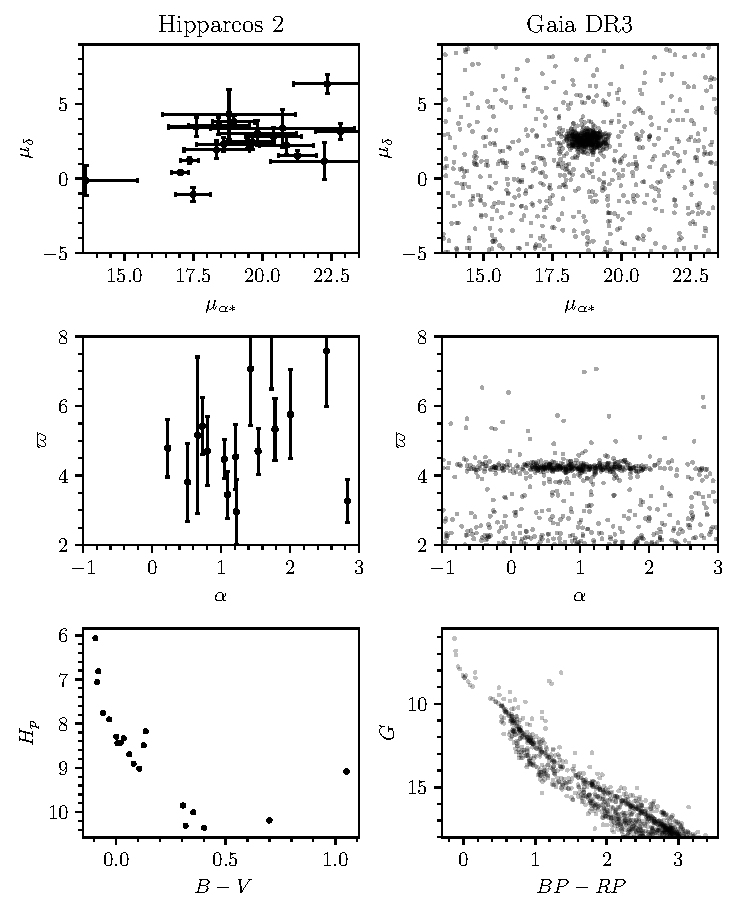
\includegraphics[width=\textwidth]{fig/c1/gaia_hipparcos_oc_comparison.pdf}
	\caption[Comparison between the regions around the star cluster Blanco~1 in data from \emph{Hipparcos} and \gaia]{Comparison between the regions around the star cluster Blanco~1 in data from \emph{Hipparcos} and \gaia. \emph{Hipparcos}-2 data \citep{vanleeuwen_hipparcos_new_2007} is shown on the left and \gaia\ DR3 data \citep{gaia_collaboration_gaia_2022} is shown on the right. The top row shows proper motions, the middle row shows parallax as a function of right ascension, and the bottom row shows the CMD of the stars in each region. While \emph{Hipparcos} only sees a few dozen bright stars for the cluster, \gaia\ can detect up to 1000, and to a significantly higher degree of astrometric accuracy.}
	\label{fig:intro:history:gaia_blanco_1}
\end{figure}

With so much data at an incredible level of quality, it is perhaps unsurprising that the OC census has been completely overhauled in just five years since the first full release of \gaia\ data (\gaia\ DR2). In many ways, \gaia\ is the perfect instrument for the study of OCs. Most OCs (such as NGC~2547 in Fig.~\ref{fig:intro:definition:comparison}) have relatively low star counts and are situated on the galactic disk, where high numbers of field stars are present -- making them challenging to isolate from background sources \citep{kharchenko_global_2012}. However, as OCs are comoving groups at a similar distance to one another and denser than the surrounding field, \gaia's proper motions and parallaxes provide an excellent way to isolate clusters from the field \citep{gaiacollaboration_gaia_data_2017,cantat-gaudin_characterising_2018}.

Figure~\ref{fig:intro:history:gaia_blanco_1} shows the region around the high galactic latitude OC Blanco~1 in data from the Hipparcos-2 catalogue \citep{vanleeuwen_hipparcos_new_2007}, compared against the same region in data from \gaia\ DR3 \citep{gaia_collaboration_gaia_2022}. The difference in precision between the two datasets is dramatic. In \emph{Hipparcos}, while the cluster is visible as an overdensity in proper motion space, in \gaia, the cluster becomes a small, compact group of stars that is trivially easy to separate from field stars. In addition, while Hipparcos parallaxes have accuracies on the order of 1~mas, \gaia's $\sim100\times$ better parallaxes make the cluster stand out as a clearly visible horizontal line as a function of right ascension. Combined together, proper motions and parallaxes make an exceptionally powerful tool to isolate OCs from field stars and derive clean, minimally contaminated membership lists. In addition, the difference in dataset size between the two telescopes is abundantly clear: \gaia\ DR3 can be used to probe the cluster eight to ten magnitudes fainter than \emph{Hipparcos}, resulting in a membership list around $\sim50\times$ larger than the cluster in \emph{Hipparcos} data. This incredible level of astrometric precision is repeated across the entire galactic disk, and has powered the last five years of revolution in the OC census.

% TODO: DR1? you may want to talk about DR1 tbh

Not long after the release of \gaia\ DR2, \cite{cantat-gaudin_gaia_2018} produced an updated catalogue of OCs and OC membership lists, using pre-\gaia\ works such as \cite{kharchenko_global_2013} as input and trying to redetect their catalogued clusters in \gaia\ data. \cite{cantat-gaudin_gaia_2018} were able to derive updated cluster membership lists with around twice as many members on average as in \cite{kharchenko_global_2013}, as well as deriving cluster proper motions to around two orders of magnitude greater precision than in \cite{kharchenko_global_2013} and precise distances to clusters.

One of the largest results of the work on the OC census so far in the era of \gaia\ has been that many clusters catalogued before \gaia\ cannot be detected in \gaia\ data. This is clear in Fig.~\ref{fig:intro:history:catalogues}, with the catalogue of \cite{cantat-gaudin_gaia_2018} containing around half as many clusters as \cite{kharchenko_global_2013}. The reasons for the non-detection of such a large number of OCs remain mostly unclear. % How can so many objects catalogued before \gaia\ be undetectable?

\cite{cantat-gaudin_clusters_2020} provided some answers to this question, searching again in \gaia\ DR2 data for some of the clusters they were unable to detect. They found that many clusters reported earlier in IR datasets continued to be undetectable in \gaia, being able to strongly rule out 38 objects as definite asterisms. The asterisms they found are generally older and at high galactic latitudes, and were typically reported in IR datasets. They comment that although \gaia's visual observations should mean some clusters are too heavily reddened to be visible to \gaia, there are nevertheless many objects that \gaia\ should still be able to detect, owing to its deep visual photometry and ease of separating OCs from the field. However, the status of at least another $\sim$1000 clusters remains unknown, with the exact reasons for their non-detection in \gaia\ being only speculation at this time. 


\subsection{New open clusters found with \gaia}
\label{sec:intro:gaia:new_clusters}

At the same time that \gaia\ has been an invaluable tool for better cataloguing already-known OCs, \gaia\ has also allowed for a large number of new OC discoveries; particularly for smaller, sparser objects that are otherwise impossible to find in 2D datasets \citep{cantat-gaudin_milky_2022}. Figure~\ref{fig:intro:history:papers} shows the approximate number of papers reporting new OCs in the 21\first\ century. Papers were found by searching the ADS\footnote{\url{https://ui.adsabs.harvard.edu/}} in Februrary 2023 for papers whose title or abstract contained the string `\texttt{new open cluster}'. The release of \gaia\ DR2 in 2018 \citep{brown_gaia_2018} clearly corresponds with the number of papers reporting new OCs each year roughly tripling.

The central challenge of finding new OCs in data from \gaia\ is the sheer size of the \gaia\ dataset, with hundreds of millions of stars to search through in a five-dimensional dataset of positions, proper motions and parallaxes for each star. While traditional approaches in the 19\third\ and 20\third\ centuries searched for clusters by hand, and works such as \cite{froebrich_systematic_2007} refined this approach by using kernel density estimation to identify overdense regions in the two-dimensional 2MASS dataset, the release of \gaia\ has also seen many new approaches for OC recovery.

% Plot of reported OCs
\begin{figure}[t]
	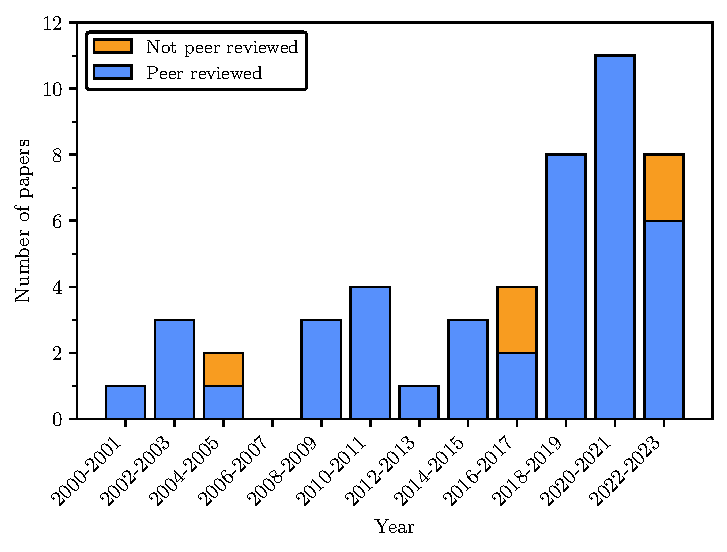
\includegraphics[width=\textwidth]{fig/c1/papers.pdf}
	\caption[The approximate number of papers reporting new open clusters in the 21\first\ century]{The approximate number of papers reporting new open clusters in the 21\first\ century, shown as a stacked bar chart of peer reviewed and non-peer reviewed works. Data for 2022-2023 are incomplete.}
	\label{fig:intro:history:papers}
\end{figure}

Machine learning (ML) has exploded into observational astronomy over the last decade, developing from a niche method into a mainstay of astronomical data analysis methods \citep{ivezic_statistics_data_2020}. ML has two primary appeals. Firstly, it mostly automates the solving of complicated problems. ML can learn the relationship between input data and a desired output largely autonomously, with the user only being responsible for checking its work. Especially for arduous tasks like classification of large datasets \citep[e.g.][]{killestein_transient-optimised_2021}, ML-based approaches can be orders of magnitude more straightforward to implement than creating a brand new algorithm or approach to solve every problem every time, or by simply solving a problem by hand as would be done traditionally. In this way, ML methods can be considered a `Swiss army knife' of model fitting, with every method being applicable to a very wide range of potential problems. Secondly, ML-based approaches are generally much quicker than previous methodologies \citep{hunt_improving_2021}, leveraging the latest computing hardware such as graphics processing units (GPUs) significantly more efficiently than previous approaches.

While ML is not without its caveats (which will be discussed later in this thesis), ML has still been essential to the dramatic increase in newly reported OCs in the \gaia\ era. \cite{castro-ginard_new_2018} were the first authors to adopt an ML-based approach for OC recovery, using two kinds of ML to automate tasks in cluster searches. Firstly, they used a clustering algorithm called DBSCAN (a form of unsupervised ML) to recover 31 new OCs in \gaia\ DR2 data, automating the process of cluster retrieval. Then, they used a neural network (a form of supervised ML) to classify OCs based on their CMD, also automating the process of assuring that OC CMDs have single stellar populations. Aside from \cite{sim_207_2019} and a handful of works where small numbers of new OCs were noticed by mistake \citep[e.g.][]{zari_3d_2018,bastian_gaia_2019,anders_ngc_2022-1}, all of the other roughly two dozen papers over the past few years that have found new OCs have used ML techniques to search for clusters.

Since then, many other works have used DBSCAN or variations on it to detect new clusters, with it proving to be an extremely popular method in the literature for OC retrieval \citep{castro-ginard_hunting_2019,castro-ginard_hunting_2020,castro-ginard_hunting_2022,liu_catalog_2019,he_catalogue_2021,he_new_2022,he_unveiling_hidden_2022,he_blind_allsky_2022,qin_discovery_2021,hao_sixteen_2020,hao_newly_2022,qin_hunting_2023}. In total, these works have reported nearly 4000 new OC candidates, which -- if all of these objects are real -- presents a major expansion in the size of the OC census. A handful of other works have used different methods, including \cite{cantat-gaudin_gaia_2019} who used Gaussian mixture models (GMMs) and \cite{jaehnig_membership_2021} who used extreme deconvolution (a probabilistic extension of GMMs).

The discovery of so many new OCs has brought a number of exciting new results. In particular, before \gaia, works such as \cite{kharchenko_global_2013} believed that the OC census of 955 objects within 1.8~kpc was largely complete; however, around $\sim$400 new OCs have been reported in this range by \gaia-based OC searches since the release of \gaia\ DR1, firmly challenging the idea that the OC census is complete at close distances and providing many new objects for study.

The most recent analysis of the completeness of the OC census in the \gaia\ era \citep{anders_milky_2020} found that the OC census within 2~kpc remains incomplete, although the full extent of this incompleteness is still an open question. It is unknown how many new OCs are remaining to be discovered and if existing methodologies could be improved upon.


\subsection{\gaia's brand new insights into open clusters}
\label{sec:intro:gaia:insights}

Although this thesis will mostly focus on methods to further improve the census of OCs, fundamentally, the reason why OCs are thoroughly important to modern observational astronomy is the science that can be performed with them. Hence, I will also quickly discuss some of the main new results into OCs that \gaia\ data has enabled, giving an overview of the power and importance of these objects.

% Plot of Meingast+ tidal tails/comas
\begin{figure}[tb]
	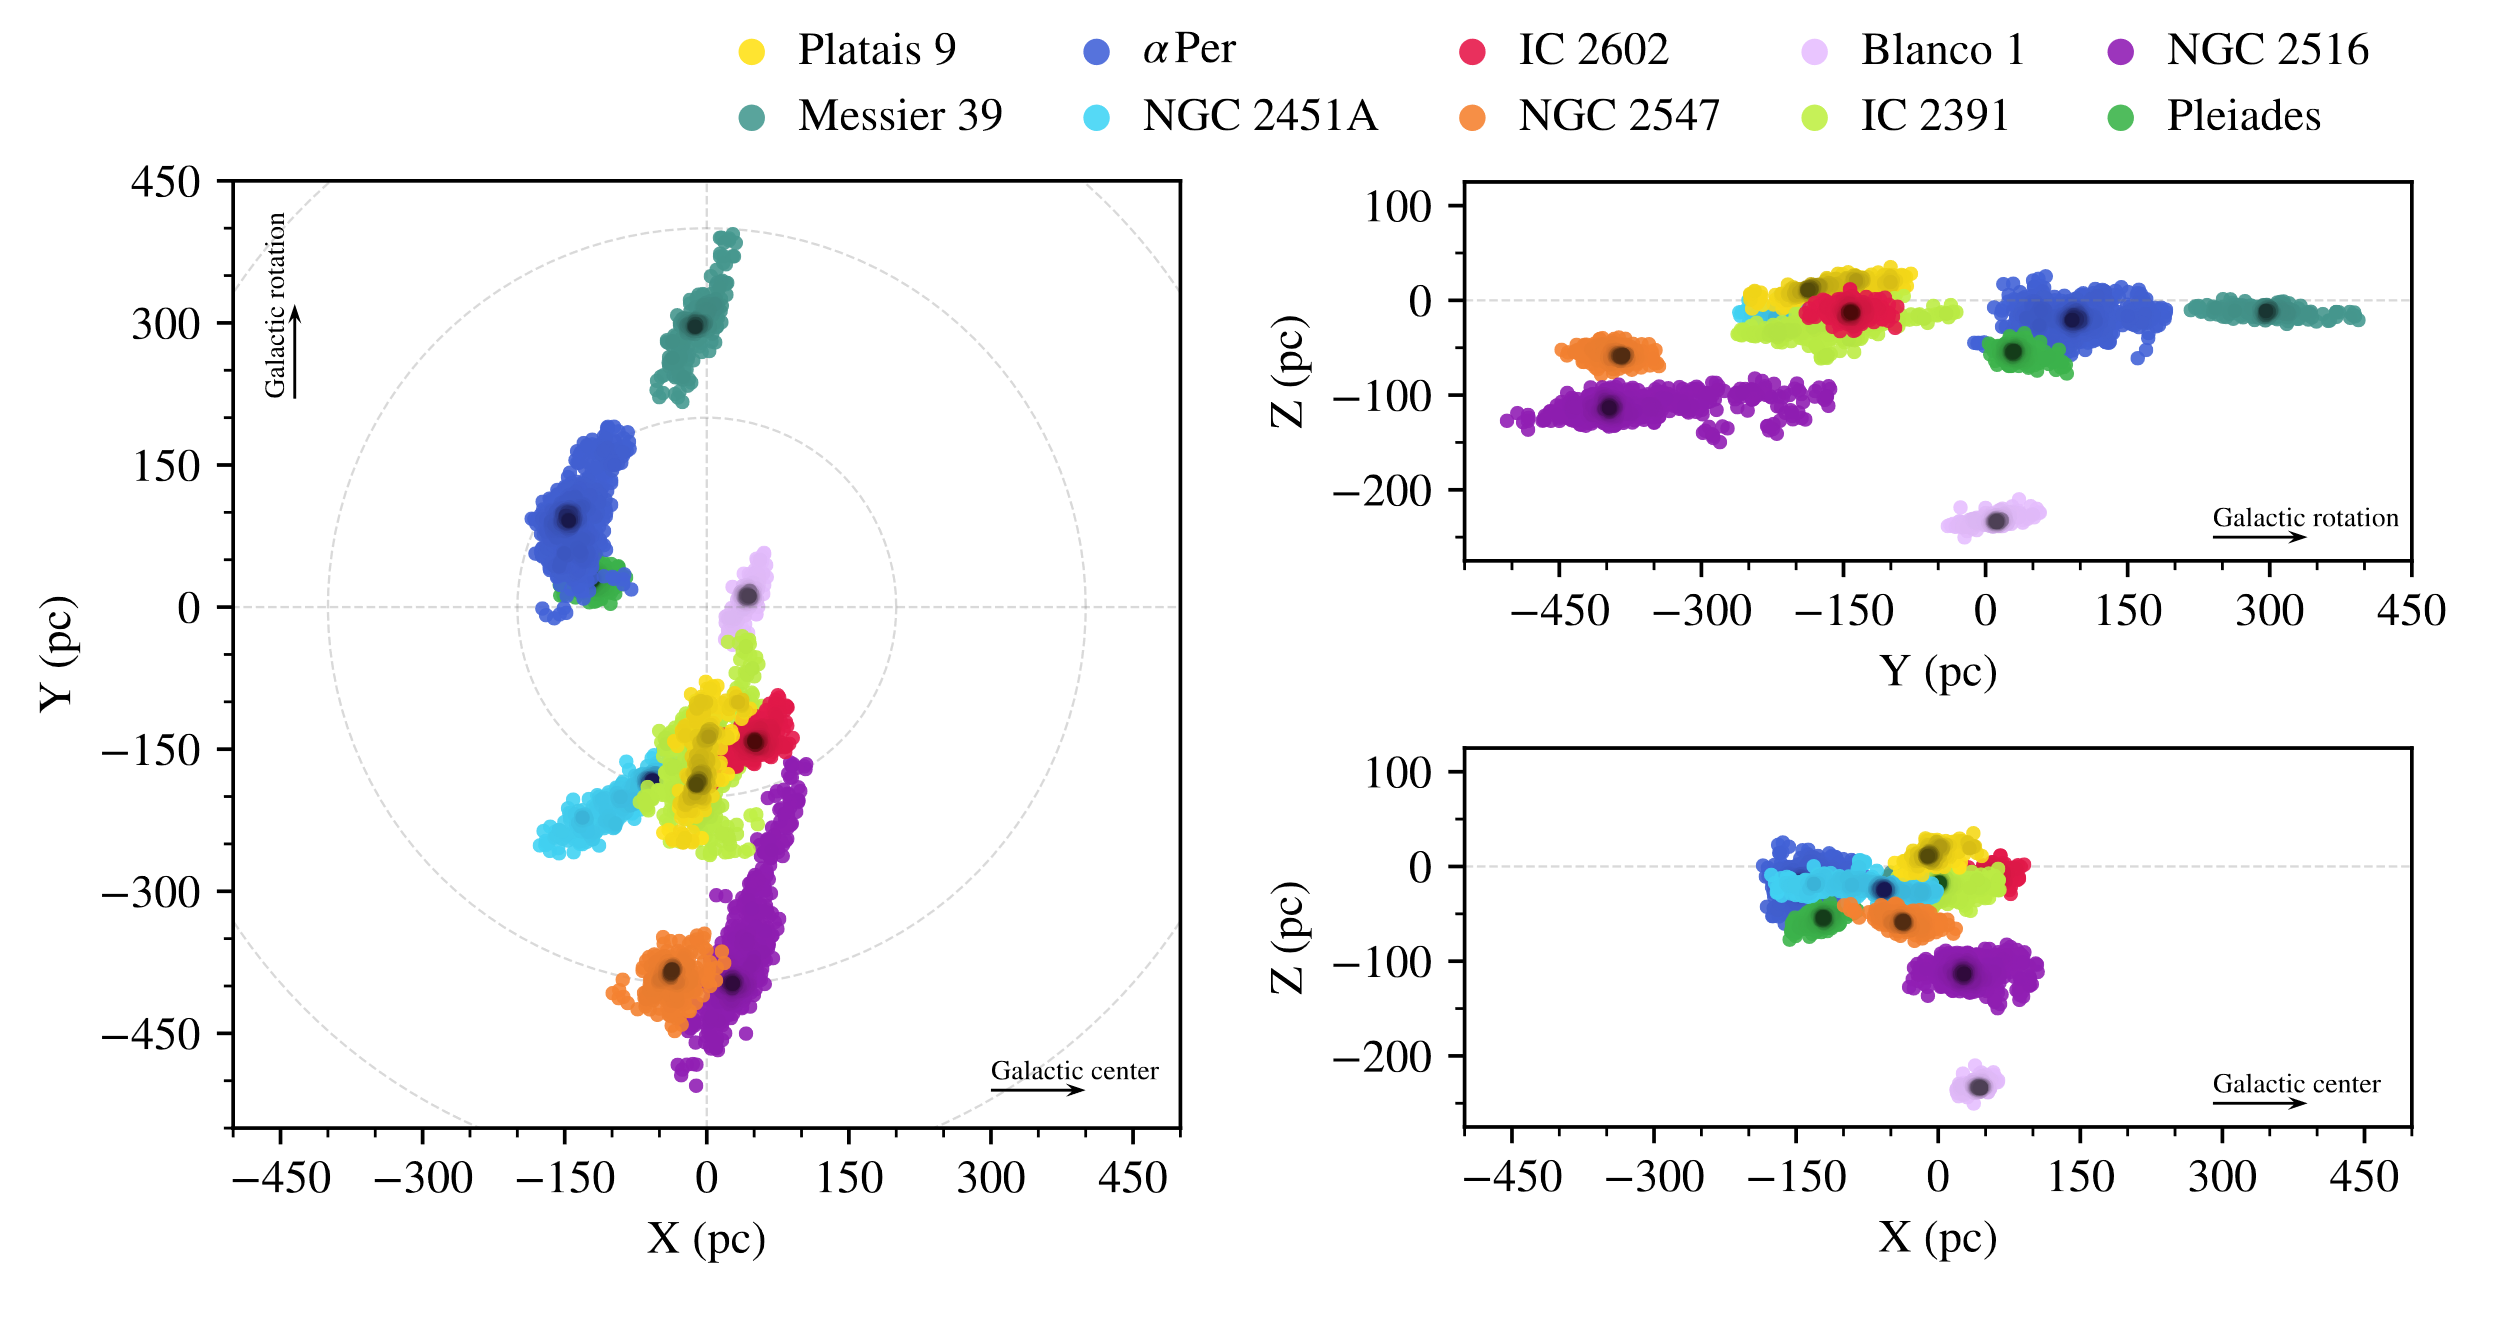
\includegraphics[width=\textwidth]{fig/c1/meingast_tidal_tails.png}
	\caption[The detected tidal tails and comas of ten OCs near to the Sun]{The detected tidal tails and comas of ten OCs near to the Sun. Clusters are shown as coloured density plots and plotted in heliocentric coordinates with the galactic centre to the right. \emph{Credit:} \cite{meingast_extended_2021}}
	\label{fig:intro:gaia:comas}
\end{figure}

One of the most exciting results of the \gaia\ era is that the dissolution of OCs can now be observed. OCs have a typical age of around 100~Myr, which is significantly younger than the $\approx 13$~Gyr age of the Milky Way, a difference that has long been argued as evidence that OCs are broken up by two-body interactions between stars ejecting some cluster members and the tidal forces of the Milky Way. Numerical simulations have shown that almost all OCs should have `tidal tails' of stars stretching in front and behind the cluster's orbit due to such interactions with the Milky Way's potential \citep{portegies_zwart_young_2010,cantat-gaudin_milky_2022}, although such tidal tails had only been observed for GCs until \gaia. Now, thanks to \gaia, the detection and study of OC tidal tails and dissolution processes is possible in exquisite detail for dozens of clusters.

As the nearest OC to the Sun, the Hyades has been extensively studied, with its spatial elongation first being probed by \cite{reino_gaia_study_2018} using \gaia\ DR1, and studied further by \cite{lodieu_3d_view_2019}, \cite{röser_hyades_tidal_2019}, and \cite{meingast_extended_stellar_2019} with \gaia\ DR2. Similar analyses have been performed on many more clusters, with \cite{meingast_extended_2021} analysing ten OCs in the solar neighbourhood and finding that not only do they all exhibit tidal tails, but most are also surrounded by `comas' of stars ejected in all directions from each cluster (Fig.~\ref{fig:intro:gaia:comas}). \cite{tarricq_structural_2022} studied 369 clusters within 1.5~kpc and detected tidal tails for 71 of them. Such clear visibility of the ongoing dynamical destruction of Milky Way OCs has been used by works such as \cite{yeh_ruprecht_2019}, \cite{oh_kinematic_modelling_2020}, and \cite{pang_3d_2021} to study the dynamics of nearby OCs and make predictions on their future lifespan. It should be possible to expand these methods to more OCs and derive dynamical parameters for a wide range of star clusters, making wide-ranging inferences about the life of star clusters after their formation.

% Plot of OC spiral arm sort-of correlation
\begin{figure}[t]
	\centering
	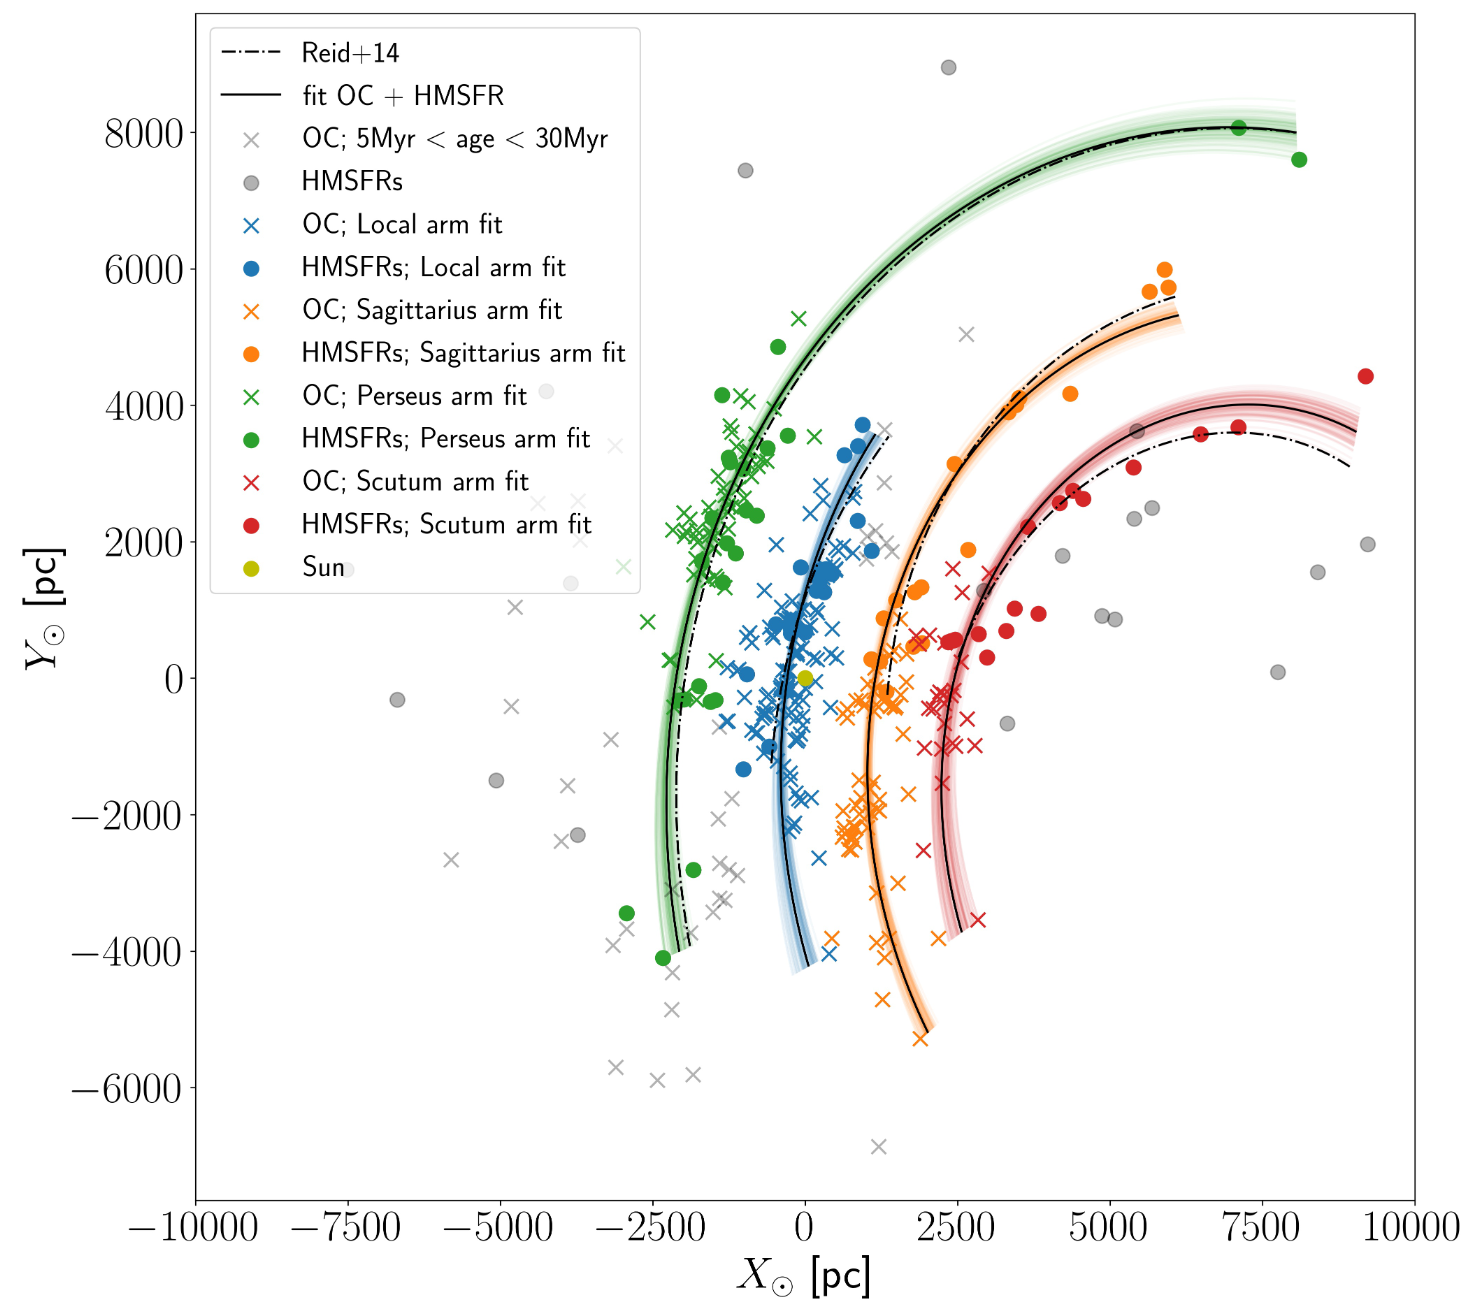
\includegraphics[width=0.8\textwidth]{fig/c1/spiral_arms.png}
	\caption[A model of the Milky Way's spiral arm structure as traced by OCs and high-mass star forming regions]{A model of the Milky Way's spiral arm structure as traced by OCs and high-mass star forming regions. \emph{Credit:} \cite{castro-ginard_milky_2021}}
	\label{fig:intro:gaia:spiral}
\end{figure}

OCs have also been extensively used to probe the wider structure of the Milky Way. \gaia's improved parallax accuracy allows for more accurate distances to OCs to be derived, and the improved OC membership lists possible with \gaia\ allow for better determination of photometric parameters. \cite{cantat-gaudin_painting_2020} derived ages, extinctions, and distances for around 2000 OCs, showing that young clusters are generally correlated towards low galactic altitudes and appear to loosely trace spiral arm models derived from masers in works such as \cite{reid_trigonometric_parallaxes_2014}, while older clusters are more uniformly dispersed and can be found at higher altitudes above or below the galactic plane, suggesting that their orbits have evolved while they aged. \cite{castro-ginard_milky_2021} used these results to perform fits of a spiral arm model to a combination of the distribution of young OCs and star forming regions (Fig.~\ref{fig:intro:gaia:spiral}), finding that the addition of young OCs slightly changes the most likely spiral arm model relative to the fit of \cite{reid_trigonometric_parallaxes_2014}.

Finally, new OC results in the \gaia\ era have allowed for a number of new studies of stellar evolution. In particular, many more exotic phases of stellar evolution can now be studied more easily thanks to \gaia\ OC membership lists, which allow for significantly easier separation of OC member stars from field contamination. 

A primary hot topic within the literature is blue straggler stars (BSSs), which are stars near to the main sequence turn-off of a cluster that are bluer and brighter than would otherwise be expected (e.g. four stars to the upper left of the turnoff point of Ruprecht~147 in Fig.~\ref{fig:intro:history:cmds}). These stars are interesting cases of non-ideal stellar evolution, with leading theories stating that BSSs may be caused by mass transfer, dynamical mergers, or a combination of multiple processes \citep{boffin_ecology_2015}. While BSSs have been extensively investigated in GCs, \gaia\ has allowed for many new investigations of BSSs in OCs \citep{cantat-gaudin_milky_2022}, such as in \cite{rain_blue_2020} who investigated BSSs in Trumpler~5, Trumpler~20, and NGC~2477, or \cite{vaidya_blue_2020} who studied BSSs in a further seven OCs and found that BSSs are not mass-segregated in just two of of the seven clusters they studied. \cite{leiner_census_blue_2021} investigated BSSs in 16 OCs and found that standard population synthesis techniques do not produce enough BSSs when compared to \gaia\ observations. They found that changes to assumptions about binary mass transfer somewhat rectify differences between observations and theoretical predictions, although they found that it still remains difficult to create the observed number of BSSs from current theories, suggesting that theories of BSS formation may still require additional physics.

Another hot topic within stellar evolution that is more easily investigated within star clusters is extended main-sequence turnoffs (eMSTOs). Initially observed only in Magellanic cloud clusters \citep[e.g.][]{bastian_effect_stellar_2009}, \gaia's improved contrast between cluster and field stars has allowed for eMSTOs to be observed in a number of Milky Way OCs \citep{marino_discovery_2018}. eMSTOs challenge traditional theories of star formation for smaller clusters such as OCs, as they could be explained by multiple stellar populations of a range of ages. On the other hand, simpler theories such as different rates of stellar rotation or even circumstellar dust are also competing theories to explain the existence of eMSTOs \citep{milone_multiple_2022,dantona_role_dust_2023}.

Finally, OCs have also been used to study and calibrate variable stars. In particular, Cepheid variable stars are a critical first rung on the cosmic distance ladder, useful for finding accurate distances galaxies within a few Mpc of the Milky Way. Currently, tension in the Hubble parameter $H_0$ could be explained in number of ways, ranging from the dominant $\Lambda$CDM cosmological model being wrong to simply being a miscalibration of one or more rungs on the cosmic distance ladder. Hence, in this context, accurate calibration and study of Cepheid variables is essential to ruling out or confirming issues with Cepheids as the source of any $H_0$ tension, a task that multiple authors have used OCs to aid in. \cite{breuval_milky_way_2020} used OCs hosting Cepheid variables to derive a new Cepheid period-luminosity relation (Leavitt law) and derive an updated value for $H_0$, finding that the Hubble constant could be revised to a lower value still in some tension with Planck CMB results \citep{planckcollaboration_planck_2018_2020} when using \gaia\ astrometry and Cepheid OC members. Works including \cite{medina_revisited_2021}, \cite{zhou_galactic_2021}, and \cite{hao_open_2022} have searched for more Cepheid variable stars within OCs to assist in the further study of Cepheids.

It goes without saying that all scientific use cases of OCs rely on the OC census being accurate, and are greatly improved by it being as complete as possible. Even though this brief review may have presented a `rosy-eyed' view of the status of OC science in the era of \gaia, there remain many issues with the current status of the OC census, with many unanswered questions and barriers to easier usability of OCs for science. In the next section, I will discuss some of these problems at length, and briefly introduce how I will try to solve some of them in the rest of this thesis.



\section{Issues and solutions for the open cluster census}
\label{sec:intro:aims}

As detailed in Sects.~\ref{sec:intro:pre-gaia} and \ref{sec:intro:gaia}, there has been a huge amount of recent scientific progress in the OC census and in the study of OCs as a whole. However, the \gaia\ era of OC science is still relatively new, with many more years of data releases being anticipated. Inevitably, this will allow for a huge range of new scientific studies into OCs \citep{gaia_collaboration_gaia_2022}. 

To maximise the scientific potential of OCs, it makes sense to improve the census of OCs as much as possible, as well as developing `future-proof' methodologies that can be applied to future \gaia\ data releases as well as the current ones. The issues with the census of OCs in the Milky Way can be divided into five broad topics that I will discuss next.


\subsection{The issues with the open cluster census}
\label{sec:intro:aims:issues}
\subsubsection{Problem 1. The methods used to detect open clusters (and their biases)}
\label{sec:intro:aims:issues:detection}

As mentioned in Sect.~\ref{sec:intro:gaia}, the \gaia\ mission has provided the OC community with a tremendous quantity of data. However, until now, many different works have tried many different approaches for OC recovery (both for recovery of existing clusters and for blind searches), with no direct comparison having been done between different approaches. Additionally, modern computer science is fast-paced, particularly in the field of machine learning. Many different approaches exist for clustering data, only a handful of which have been trialed for OC recovery \citep{xu_comprehensive_2015}, despite the fact that publically available open-source implementations of these algorithms are often available and ready to use \citep[e.g.][]{scikit-learn}.

This causes a number of problems. Primarily, it is unclear whether or not existing approaches are subject to biases. Particularly since almost all blind searches for OCs have used DBSCAN (Sect.~\ref{sec:intro:gaia:new_clusters}), it could be that a bias with the algorithm could prevent certain clusters from being detected depending on their age, distance, or other parameters, which may mean that a whole type of new OC has been as-yet undiscovered within \gaia\ data. There is no certainty that all OCs that \emph{can} be detected \emph{have} been detected with \gaia.

It is also unclear how many false positives current approaches produce. Most works do not include an estimate of how many of their reported clusters are real \citep[e.g.][]{castro-ginard_new_2018,liu_catalog_2019,he_catalogue_2021}. It is not known whether or not it is safe to assume that the results of a clustering algorithm can always be trusted, and it is not known whether certain algorithms are more or less trustworthy.

Additionally, there are many quirks with the usability of current approaches. For instance, the comprehensive DBSCAN-based works of \cite{castro-ginard_new_2018,castro-ginard_hunting_2019,castro-ginard_hunting_2020,castro-ginard_hunting_2022} adopted a sky tiling scheme that requires a large number of algorithm re-runs, resulting in a method that must be applied on a supercomputer \citep{castro-ginard_hunting_2022}. It is not known whether a more efficient approach that requires fewer computational resources and is easier to repeat on future data releases is possible. This is a particular issue as future \gaia\ data releases are likely to contain higher numbers of reliable sources \citep{gaia_collaboration_gaia_2022}, meaning that current approaches will need to be ran on four to eight times as many sources\footnote{Calculated for \gaia\ DR3, which contains $\sim$250 million sources with $G\leq18$, which is a commonly adopted cut; however, the final \gaia\ data release is projected to contain at least 1 billion sources \citep{gaia_collaboration_gaia_2016}.}.


\subsubsection{Problem 2. The status of clusters discovered before \gaia}
\label{sec:intro:aims:issues:pre_gaia}

Of the many clusters discovered before \gaia, fewer than 50\% have so far been re-detected in \gaia\ data \citep{cantat-gaudin_gaia_2018,cantat-gaudin_clusters_2020}. The fact that so many objects are missing from \gaia-based OC studies could represent a total paradigm shift in the census of OCs in the Milky Way, or it could be indicative of the limitations of \gaia. For every cluster, there are two possibilities.

In the case that an object is real but cannot be detected in \gaia\ data, such as for heavily reddened clusters discovered using IR datasets that are obscured by dust in \gaia\ data \citep{cantat-gaudin_clusters_2020}, such an object would be a sign of the incompleteness of the \gaia\ OC census. If a significant number of IR clusters are in fact real, then to study all known OCs, it would be necessary to use both \gaia\ and IR datasets simultaneously.

On the other hand, it is also possible that such objects are not real. \gaia\ has significantly higher astrometric accuracy than all previous astrometric catalogues, and \gaia\ should be sensitive to a large number of real OCs, even for those with intermediate levels of reddening \citep{cantat-gaudin_clusters_2020}. 

While some studies have performed small investigations into clusters missing from \gaia\ on a case-by-case basis \citep[e.g.][]{cantat-gaudin_clusters_2020,piatti_catching_2023}, the status of most objects is still unknown. It should be possible to rule out many OCs reported previously in the literature given a large enough study. Alternatively, if \gaia\ is in fact a major limitation in recovering many OCs discovered before \gaia\ using IR datasets, then different datasets would need to be used to study such objects. This would also be a further strong science case for \gaia\ follow-up missions such as the proposed \emph{GaiaNIR} mission for near-infrared astrometry \citep{hobbs_gaianir_combining_2016}.


\subsubsection{Problem 3. The status of clusters discovered with \gaia}
\label{sec:intro:aims:issues:post_gaia}

At the same time as the aforementioned `re-detection crisis' of clusters reported before \gaia, thousands of new OC candidates have been reported in the literature. Most of these objects have not been independently verified \citep{cantat-gaudin_milky_2022}, meaning that a large number of objects exist in the literature and may be being used for studies of OCs and galactic structure but without knowing which objects are or are not real \citep[e.g.][]{anders_milky_2020,castro-ginard_milky_2021}. Given that so many clusters cannot be detected from recent works reporting new OCs before \gaia, with some works such as \citep{scholz_global_2015} having as many as 100\% of their clusters being impossible to redetect \citep{cantat-gaudin_gaia_2018}, it is not far-fetched to suggest that there can be reproducibility issues between different studies when reporting new objects. Hence, there is a need to independently verify new OC candidates reported recently using \gaia\ data, preferably also with an alternative methodology and a thorough analysis of which objects are and are not real.

Additionally, it is also possible that some objects reported recently are duplicates. The large number of papers reporting new OCs since the release of \gaia\ DR2 (Fig.~\ref{fig:intro:history:papers}) can make the literature difficult to keep up with \citep{cantat-gaudin_milky_2022}. There is likely a need to verify that new cluster candidates are unique and have not been previously reported in the literature. For instance, during the writing of this thesis, \cite{chi_blind_search_2023} (accepted in ApJS) reported 1179 new OCs, which would represent a large increase in the number of newly discovered OCs in the \gaia\ era. However, many plots of their `new' clusters are clearly compatible with OCs previously reported in the literature (e.g. candidate 14677, which is Blanco~1). The existence of works containing duplicates `muddies the water' when attempting to use existing catalogues of OCs in combination with papers reporting new objects. There is a clear need to verify that newly reported OCs are real, unique clusters. 


\subsubsection{Problem 4. The completeness of the \gaia\ open cluster census}
\label{sec:intro:aims:issues:completeness}

Despite the publication of many works that have used \gaia\ data to report thousands of new OCs (Sect.~\ref{sec:intro:gaia:new_clusters}), it is still unclear how complete the \gaia\ census of OCs is. It is not clear how many objects are missing or if any further biases contribute to certain objects being missed. Beyond the widespread disproving of the result in \cite{kharchenko_global_2013} that the OC census is complete within 1.8~kpc, there has been little study in the \gaia\ era on the completeness of the OC census.

Nevertheless, the completeness of any catalogue, not least the OC census, is an interesting thing to know that would enable a large number of scientific studies. The study of star clusters in the Milky Way is unique in that we are able to study bound star clusters of significantly lower masses and luminosities than is possible in extragalactic studies \citep{portegies_zwart_young_2010}. While extragalactic astronomy is able to probe the occurence rates of massive, highly luminous clusters in a large number of galaxies, it is only in the Milky Way that study of low-mass objects is possible, due to their low luminosity. Milky Way OCs are hence an important calibration point for understanding star formation at lower mass ranges.

Given that the Milky Way's cluster age and mass functions are uniquely important in the general study of star clusters, it is vital that the completeness of the OC census can be well known. Although this has been attempted in \gaia\ data by \cite{anders_milky_2020}, who also derive a completeness estimate of the OC census, their work has two main limitations. Firstly, they used the blind searches of \cite{castro-ginard_new_2018,castro-ginard_hunting_2019,castro-ginard_hunting_2020} to calibrate their completeness function. However, it is not known if the DBSCAN algorithm used in these works has any biases that their completeness estimate would inherit (see Problem~1/Sect.~\ref{sec:intro:aims:issues:detection}). Secondly, they only create a selection function in terms of cluster age and distance. They expect that other parameters, such as cluster mass or size, could be major factors in the OC selection function. They were unable to include mass in their selection function due to the lack of cluster mass measurements in the \gaia\ era.

In addition, it is not clear how many more new OCs could be detected with future \gaia\ data releases. In theory, it should also be possible to extend such a prediction to other proposed surveys and instruments such as \emph{GaiaNIR} \citep{hobbs_gaianir_combining_2016}. Given that the proposals for \emph{GaiaNIR} describe science with OCs as a key scientific justification for the mission, a way to predict how many OCs would be discovered by a near-infrared astrometric mission such as \emph{GaiaNIR} would be an interesting way to strengthen the science case for future astrometric missions and surveys.


\subsubsection{Problem 5. The observational definition of open clusters}
\label{sec:intro:aims:issues:definition}

Finally, and somewhat amusingly, possibly the greatest issue with the OC census in the \gaia\ era is that no work can agree on what OCs actually are (at least observationally). While the theoretical definitions of star clusters in the Milky Way can now be reasonably clearly defined \citep[Sect.~\ref{sec:intro:definition}][]{portegies_zwart_young_2010}, it is challenging to convert these theoretical definitions into a firm observational definition for OCs. Critically, this presents a number of issues when comparing between different works or when trying to combine the results of separate OC studies.

Most works reporting new OCs use different quality criteria to decide which objects are or are not included in their work. Almost all use some sort of criteria on colour-magnitude diagrams, requiring that the cluster CMD is narrow and compatible with a single stellar population. However, this is implemented in many different ways; including by using statistical criteria \citep[e.g.][]{liu_catalog_2019}, a neural network classifier \citep[e.g.][]{castro-ginard_new_2018}, or simple manual classification \citep[e.g.][]{he_catalogue_2021}. Some works require that clusters are clear statistical overdensities in \gaia, deriving something analogous to a signal to noise ratio (S/N) for their cluster candidates \citep[e.g.][]{cantat-gaudin_gaia_2019}. Some works also limit clusters based on their physical parameters, requiring that they are compact groups and hence more likely to be gravitationally bound \citep[e.g.][]{liu_catalog_2019}. Finally, all works adopt a different minimum size for an OC, ranging from as low as 8 stars \citep{castro-ginard_new_2018} to as high as 50 \citep{liu_catalog_2019}. With so many differing definitions of what constitutes a good enough OC candidate, it can be difficult to compare the results of multiple works or to combine them into singular catalogues without introducing biases. In addition, most works use simple binary `yes/no' cuts on whether or not an OC passes a given constraint, which may not capture all of the uncertainty inherent in deciding whether an edge-case object is or is not a real OC.

\cite{cantat-gaudin_clusters_2020} outlined a set of empirical criteria to follow that all new OC candidates should meet, requiring that OCs are a clear overdensity in astrometric data, that they have a CMD with a clear homoegeneous population of stars, and that the cluster meets two cuts on its parameters intended to be a comparable test for being bound: that the radius containing 50\% of members is smaller than 20~pc, and that the cluster's proper motion dispersion corresponds to an internal velocity dispersion of less than 5~kms\textsuperscript{-1}. While these criteria are an empirical minimum for an OC, as a thought experiment, it is still relatively straightforward in a dense region of the galactic disk to find $\sim$10 or more stars within 40~pc of each other and with a velocity dispersion below 5~kms\textsuperscript{-1}, and so these criteria are not infallible, and could allow unbound moving groups to be misclassified as OCs.

A `gold standard' observational definition of an OC might be more directly derived from the theoretical definition presented in Sect.~\ref{sec:intro:definition} -- requiring that an OC is an overdensity, a single stellar population, and is unambiguously gravitationally bound. However, no such way to measure such parameters for a large number of clusters exists, principally due to the difficulty in measuring the dynamics and boundness of a large catalogue of star clusters.


\subsection{The aims of this thesis}
\label{sec:intro:issues:aims}

Even relative to the major improvements to OC science in the 1990s and 2000s, \gaia\ has still been utterly groundbreaking in the quality and quantity of data it provides on our galaxy. Never before has so much precise data been available for so many stars; \gaia\ will rewrite textbooks on the composition and characteristics of the Milky Way. Within the field of OCs, this is clear from the many incredible new \gaia\ results highlighted in Sect.~\ref{sec:intro:gaia}. Yet as the many problems discussed in the previous section show, many issues remain with the census of OCs. In this thesis, I hope to showcase timely research that can present solutions or partial solutions to the above problems, developing the methods used to analyse OCs in the \gaia\ era to maximise the scientific potential of these objects.

First and foremost, it is impossible to solve many of the other issues in the OC census without an understanding of the limitations and biases inherent to different methods for OC retrieval (Problem 1). In addition, numerous unexplored methods for cluster retrieval present in the computer science literature could provide better options for the recovery of OCs \citep{xu_comprehensive_2015}. To date, there has been no comparative study into the advantages and disadvantages of different approaches for cluster retrieval, despite the clear importance of understanding the limitations of different methods; hence, the first part of this thesis focuses on trialing different algorithms for OC recovery in \gaia\ DR2 data, performing a comparative study into their effectiveness. In this study, I will also aim to find optimal ways to divide \gaia\ data for OC retrieval, aiming to present a method that can be ran efficiently even on larger datasets, allowing for more sources to be incorporated in the future as \gaia\ data releases improve. In the best case scenario, a method can be found that can redetect the clusters reported by all other works with minimal bias.

With a best method found, other problems in the census will be more straightforward to solve. Finding the best methodology for OC retrieval and knowing its biases will allow for the application of the method to solve Problems 2 and 3, and to a lesser extent Problem 4. Specifically, in the second study of this thesis, I conduct a large-scale unbiased blind search for OCs using the best method found and data from \gaia\ DR3. Depending on which \gaia-discovered clusters can be found in this search and depending on the effectiveness of the method found in the first study, it will be relatively simple to solve Problem 3, as some clusters will (or will not) be possible to re-detect. This study will conduct the largest validation of OCs discovered using \gaia\ to date.

An unbiased all-sky search will also allow for a solution to Problem 2. Previously, studies have generally focused on small, case-by-case attempts to retrieve OCs that were originally catalogued in pre-\gaia\ works \citep[e.g.][]{cantat-gaudin_clusters_2020}. However, an all-sky search ought to recover all OCs visible in \gaia\ within the limitations of the adopted methodology; given the understanding of this methodology gained from the first study, it should be possible to say with reasonable certainty whether or not \gaia\ should be able to detect many of the as-yet undetected OCs from before \gaia. This will greatly aid in bridging the OC census from pre-\gaia\ works to the \gaia\ era, tracing down any remaining missing clusters while suggesting that some are not real.

Inferring the completeness of the OC census is a major task, which this thesis will contribute towards but may not completely solve. An unbiased all-sky blind search for OCs is a good tool to find as many OCs as possible and reduce the incompleteness of the OC census. Despite the many works that have already searched for new OCs (Sect.~\ref{sec:intro:gaia:new_clusters}), there may still be many new objects left to discover. This search can be used as a drop-in replacement for the methodology of e.g. \cite{anders_milky_2020}, serving as a better `experiment' to detect a large sample of OCs. However, given that cluster masses are expected to be a major contributor to the selection function of OCs in \gaia, with less massive clusters being more difficult to detect, it will also be important to calculate accurate cluster masses for the entire sample of objects from the blind search. The final study of this thesis partly focuses on calculating cluster masses, which will help to solve Problem 4 while also deriving a generally useful parameter for OCs that has never been derived for such a large catalogue before. Cluster masses also require cluster ages, which I aim to derive estimates of in the second study to accompany the overall OC catalogue.

Finally, Problem 5 is likely to continue to plague the OC community for years to come, owing to the complexity of precisely defining OCs observationally. However, throughout this thesis, I will present new methods to try and convert a theoretical, first-principles oriented definition of an open cluster into a practical observational method to classify objects as OCs, MGs, GCs, false positives, or somewhere inbetween one of those categories. I aim to do so statistically, never presenting simple binary probabilities of an object being a false positive or one of the classes of real star cluster, but rather using a statistical treatment to aid in the definition of edge-case objects that could be between different classes. In the first study of this thesis, I augment clustering algorithms by trialing a number of different tests for the density of a cluster compared to its field, deriving a simple and efficient test of a cluster's astrometric signal to noise in \gaia\ data. In the second study of this thesis, I use an approximately Bayesian neural network to classify the likelihood of an OC being compatible with a single stellar population given the predictions of stellar evolution models. In the final study of this thesis, I present a preliminary method to test the boundness of OC candidates and ascertain if they are a real bound object or simply an MG.

In total, with this thesis, I hope to contribute to the difficult task of cataloguing and characterising the OCs of the Milky Way in the era of \gaia. Implicitly, all of these methods will be `future-proof' and applicable to future \gaia\ data releases, or future surveys that could replace the \gaia\ telescope. Inevitably, no method is perfect, and I will conclude by speculating on future avenues of research that could further develop the methods used to analyse OCs.


Before launching into the scientific content of this thesis, it is important to also present some theoretical background into OCs.


% ---------------------------------------
\section{Further background into star clusters and associated common methods}
\label{sec:intro:theory}

To improve the reach and readability of this thesis, I feel it is important to review some common techniques and pieces of theory from the literature. For the seasoned open cluster astronomer, this section could be browsed quickly; for the non-specialist, I hope that this section provides more insight into pieces of theoretical knowledge that I will assume for the scientific parts of this thesis.

I begin by going into more depth on some of the most important methods to OC observers.


\subsection{Analysis of CMDs}
\label{sec:intro:theory:cmds}

% Plot of CMDs of OCs
\begin{figure}[tb]
	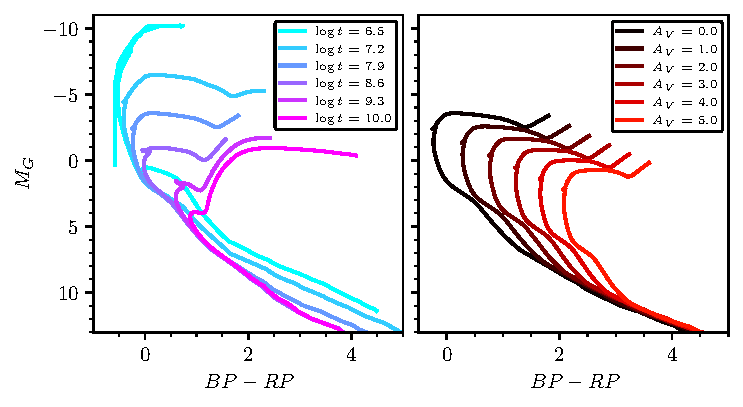
\includegraphics[width=\textwidth]{fig/c1/isochrones.pdf}
	\caption[A comparison between stellar isochrones of various different parameters.]{A comparison between stellar isochrones of various different parameters, derived from PARSEC stellar evolution models \citep{bressan_parsec_2012} and shown in \gaia\ photometric bands. \emph{Left:} isochrones of solar metallicity and zero extinction shown for six different ages. Most noticeably, as cluster age increases, the magnitude of the turn-off point decreases, with ever-more stars evolving into red giants and eventually reaching the end of their lives. The rest of the stars in the cluster also move down slightly, relaxing onto the main sequence as they age. \emph{Right:} the $\log t = 7.9$ isochrone from the left plotted at a range of different extinction values. Extinction reddens cluster stars as well as reducing their overall brightness. Extinction in \gaia\ photometry has a strong affect on the location of the turn-off point.}
	\label{fig:intro:history:isochrones}
\end{figure}

As discussed previously, CMDs are essential tools to derive many key parameters of a star cluster (Fig.~\ref{fig:intro:history:cmds}). The most common method to determine the age, extinction, and to a lesser extent the distance of a cluster is by fitting isochrones to cluster CMDs. An isochrone gives the predicted colour and luminosity of a population of stars with a range of masses given that the stars have the same age, extinction, composition, and distance. Stellar isochrones are derived from stellar evolution models such as PARSEC \citep{bressan_parsec_2012} and are widely used in many areas of observational astronomy.

In practice, isochrones are difficult to fit, with age, extinction, distance, and metallicity all being somewhat degenerate with one another. Figure~\ref{fig:intro:history:isochrones} shows the effect of varying age and extinction on stellar isochrones, with both age and extinction moving the location of the cluster turn-off point. Cluster distance merely shifts the isochrone up or down based on the cluster's distance modulus, although this is still slightly degenerate with age and extinction. Finally, the chemical composition of a cluster (most often parameterised with its metallicity $\left[\text{Fe}/\text{H}\right]$) has the smallest impact on cluster isochrones and is not shown, but will nevertheless slightly impact age and extinction determination.

Isochrone fitting is further complicated by the presence of other cluster features, such as blue stragglers, eMSTOs, or the presence of a binary sequence due to unresolved binaries (see binary sequences in Fig~\ref{fig:intro:history:cmds}, showing a clear second line of stars sat slightly above the main cluster population).

Probably unsurprisingly, there are hence many methods used in the literature to fit isochrones to data. Particularly as computational power is a major hindrance to performing three or four-parameter fits with stellar isochrones, historically, it was common to simply fit isochrones by hand, which includes no robust uncertainty estimate and can open the door to human biases. For instance, the isochrones in \cite{kharchenko_global_2013} were fit by eye, minimising $\chi^2$ goodness-of-fit criterions manually. \cite{yen_reanalysis_2018} developed this methodology further to perform $\chi^2$ fitting of all cluster parameters autonomously. \cite{hippel_inverting_2006} created a full Bayesian methodology to fit isochrones to cluster CMDs, which has been used by works in the \gaia\ era such as \cite{bossini_age_2019}.

By far the main flaw of cluster isochrone fitting is speed. Three or four-parameter fits using complicated stellar isochrones simply cannot be performed quickly, requiring significant amounts of computation time to complete in e.g. \cite{yen_reanalysis_2018}, making these key cluster parameters relatively time-intensive to derive using traditional isochrone fitting techniques. Alternatively, a recently developed approach used in \cite{cantat-gaudin_painting_2020} and \cite{kounkel_untangling_2020} uses neural networks trained on the results of a small subsample of precise isochrone fitting results for OCs to derive ages, extinctions, and distances to clusters. This uses significantly less computational time, although with the disadvantage that a subset of isochrone fits must be first created to then use as a training dataset.


\subsection{Radial profiles}
\label{sec:intro:theory:profile}

The physical size of OCs is another important property that can be measured. The size of observed clusters can be compared against theoretical predictions, and interesting relationships between parameters such as the size of clusters as a function of their age can be determined \citep{tarricq_structural_2022}.

The simplest commonly used measure of the size of an open cluster is the radius containing 50\% of members, $r_{50}$, which is the median radius of all detected member stars from the cluster centre. This radius has been commonly measured in the literature for OCs \citep[e.g.][]{cantat-gaudin_gaia_2018,cantat-gaudin_clusters_2020}. For a cluster where the mass of member stars is not correlated with their position in the cluster, such that high and low mass stars are equally distributed throughout the cluster (i.e., the cluster is not mass segregated), $r_{50}$ is equivalent to a common theoretical definition -- the half-mass radius $r_{hm}$, a radius commonly measured in theoretical works due to its use in various dynamical equations \citep{portegies_zwart_young_2010}.

However, simple measures of cluster radius are not informative about the shape of a cluster, as clusters have long been known to have different shapes, with some clusters being more centrally concentrated in their `core' and others being sparser. It is helpful to apply models to OC radial profiles, allowing for the shape of clusters to be compared given models of a small number of parameters.

\cite{king_structure_star_1962} models are the most common models applied to star clusters. While originally derived for GCs, these models have also been shown to be a good fit to many OCs \citep[e.g. in ][]{piskunov_towards_2007}, with a radial distribution function $f$ given by:

\begin{equation}
	f = k \left\{ \frac{1}{\sqrt{1 + \left(r/r_c\right)^2}} - \frac{1}{\sqrt{1 + \left(r_t/r_c\right)^2}} \right\}^2
\end{equation}

\noindent
where $r$ is the distance from the cluster centre, $r_c$ is the radius of the core of the cluster (the radius at which the surface density drops to half that of the centre), and $r_t$ is the tidal radius of the cluster beyond which the Milky Way's potential is dominant. This can also be convenient to express in terms of the total number of stars within a distance $r$ from the center of a cluster $n(x)$, which is given by:

\begin{equation}
	n(x) = \pi r_c^2 k \left[ \ln(1+x) - 4 \frac{\sqrt{1+x} - 1}{\sqrt{1 + x_t}} + \frac{x}{1 + x_t} \right]
\end{equation}

\noindent
where $x = (r / r_c)^2$ and $x_t = (r_t / r_c)^2$. Within the tidal field of a galaxy (such as the Milky Way), it is also helpful to compare the King tidal radius with the theoretically predicted Jacobi radius of a spherically symmetric cluster $r_J$:

\begin{equation}
	r_J = \left( \frac{GM}{4\Omega^2 - k^2} \right)^{\frac{1}{3}}
	\label{eqn:intro:jacobi_radius}
\end{equation}

\noindent % https://astronomy.stackexchange.com/questions/26099/jacobi-vs-tidal-radius-for-star-cluster
which relates the limiting radius of a cluster's potential field (its Roche surface) $r_J$ to the cluster's mass $M$, given the circular frequency $\Omega$ and the epicyclic frequency $k$ of the cluster's orbit. Stars outside of $r_J$ are no longer bound to the cluster, with the galaxy's gravitational potential instead being dominant. For a spherically symmetric cluster on a circular orbit, $r_J \approx r_t$, relating a cluster's mass to the product of a King model fit (or vice versa) \citep{binney_galactic_1987}. Works including \citep{piskunov_tidal_2008} have used this relation to derive cluster masses from King model fits.

As an empirical model, the \cite{king_structure_star_1962} model is mostly useful for simple observational comparisons between clusters, such as comparisons between the core and tidal radii between clusters of different ages \citep{kharchenko_global_2013,tarricq_structural_2022}. \cite{king_structure_1966} re-derives a similar model from theoretical principles, including by assuming that the velocity distribution of stars in the centre of a star cluster is isothermal and that the cluster is in virial equilibrium. The shape of these models is parameterised by a dimensionless variable $W_0$ which parameterises the concentration of a cluster, with higher values corresponding to a more centrally concentrated cluster. For $W_0 \lesssim 7$, \cite{king_structure_star_1962} and \cite{king_structure_1966} models are very similar. In practice, almost all OCs have $W_0 < 7$, and so these models can be used somewhat interchangeably \citep{portegies_zwart_young_2010}. Due to the significantly simpler functional form of \cite{king_structure_star_1962} models, they are used almost exclusively in the OC literature relative to \cite{king_structure_1966} models \citep{portegies_zwart_young_2010,cantat-gaudin_milky_2022}.

Finally, it is worth mentioning the model of \cite{plummer_problem_1911}. Once again originally designed for GCs, this model parameterises how centrally concentrated a star cluster is based on a single scale factor $a$. Unlike \cite{king_structure_star_1962} and \cite{king_structure_1966} models, the \cite{plummer_problem_1911} model assumes star clusters do not have a physical limiting radius and extend to infinity, which is of course unrealistic. Nevertheless, the \cite{plummer_problem_1911} model is still a satisfactory approximation of star cluster distribution functions, and it is still used in the literature due to its simple functional form for which many parameters can be solved analytically \citep{dejonghe_completely_analytical_1987}. \cite{plummer_problem_1911} models are particularly popular in theoretical studies of star clusters due to this reason \citep{portegies_zwart_young_2010}.


\subsection{Dynamics}
\label{sec:intro:theory:dynamics}

Later in this thesis, I use measures of OC dynamics to test if OCs are bound. Some works such as \cite{bravi_gaia-eso_2018} and \cite{pang_3d_2021} have used similar methods on small scales to test if OCs are bound. The following useful definitions are all from \cite{portegies_zwart_young_2010}.

Firstly, for a cluster with a one-dimensional velocity dispersion $\sigma_\text{1D}$, its total kinetic energy $T$ is approximately

\begin{equation}
	T = \frac{3}{2} M \sigma_\text{1D}^2
\end{equation}

\noindent
where $M$ is the total cluster mass. In addition, one can define the total potential energy of a cluster $U$ as 

\begin{equation}
	U = - \frac{GM^2}{2r_\text{vir}}
\end{equation}

\noindent
where $G$ is the gravitational constant and $r_\text{vir}$ is the theoretically definied virial radius of the cluster, a parameter that is difficult to calculate observationally as it requires three-dimensional positions. The three-dimensional virial radius can be converted to the two-dimensional deprojected median radius $r_{50}$ with

\begin{equation}
	r_\text{vir} = \frac{\eta}{6} r_{50}
\end{equation}

\noindent
where $\eta$ is a constant that is model-dependent. For an ideal \cite{plummer_problem_1911} model, $\eta$ is equal to 9.75, although in practice, this value can be out by a factor of two to four in extreme cases of star clusters with distributions that are poorly described by a \cite{plummer_problem_1911} model \citep{portegies_zwart_young_2010}.

Finally, putting these together, one can define the virial ratio $Q$ of a cluster, which is the ratio of kinetic to potential energy for a given bound system. Since the virial theorem predicts that $2T + U = 0$, $Q$ is hence given by

\begin{equation}
	Q = \frac{T}{\left| U \right|}
	  = \frac{\eta r_{50} \sigma_\text{1D}^2}{2GM}
	  \approx \frac{1}{2} \quad \text{for a bound cluster.}
	\label{eqn:intro:virial_ratio}
\end{equation}

\noindent
Equation~\ref{eqn:intro:virial_ratio} is also commonly expressed in terms of the predicted one-dimensional velocity dispersion of a virialised cluster $\sigma_\text{vir}$ for a cluster of a given mass and radius \citep[e.g. in][]{bravi_gaia-eso_2018}, as

\begin{equation}
	\sigma_\text{vir} = \sqrt{\frac{GM}{\eta r_{50}}}.
	\label{eqn:intro:virial_velocity}
\end{equation}

With these equations and measures of cluster mass, radius, and velocity dispersion, it is possible to probe the overall dynamical state of a cluster observationally or in the result of simulations \citep{banerjee_how_2017,bravi_gaia-eso_2018,pang_3d_2021}.


% \subsection{Timescales}
% \label{sec:intro:theory:timescales}

\subsection{Formation, evolution and destruction}
\label{sec:intro:theory:evolution}

Finally, having considered various individual pieces of important theory, it is also worth discussing the current overall theory of star cluster formation and evolution, which should give some theoretical context to the clusters observed at different ages in this work.


\subsubsection{Formation (up to \textasciitilde1 Myr)}

As discussed previously, stars form when clouds of cold molecular gas (giant molecular clouds, GMCs) within galaxies collapse due to gravity. This process is not believed or observed to be continuous: stellar winds from young stars rapidly heat and blow away any remaining gas within the cluster, preventing further star formation from occuring. Effectively, this process `freezes' star formation, ensuring that the resulting group of stars is roughly homogeneous in age and chemical composition \citep{lada_embedded_2003,krumholz_how_2020}. If the parent GMC is dense enough, then the stars will eventually collapse into a bound star cluster \citep{portegies_zwart_young_2010,krumholz_star_2019,krumholz_how_2020}. GMCs in the local universe generally have masses in the range $\sim10^3$ to $\sim10^7$~\MSun \citep{krause_physics_2020}. For exceptionally large GMCs with masses in excess of $\sim10^8$~\MSun, it is believed that they are large enough to form clusters as massive as GCs. Such conditions are rare in the current universe, being much more common at redshifts $z \gtrsim 2$ \citep{krumholz_star_2019}; such high-mass GMCs and the clusters they form are hence outside of the range of open clusters in this study, which generally have ages of no more than $\sim$1~Gyr. 

Historically, it was believed that all stars formed in bound star clusters. However, recent observations with \gaia\ have suggested that it may only be a minority of stars that form in bound clusters \citep{ward_not_2019,wright_ob_associations_2020}. Nevertheless, for GMCs that are dense enough to at least form an OC, a bound, virialised young cluster will emerge.


\subsubsection{Supernova feedback and expansion (\textasciitilde1 to \textasciitilde30~Myr)}

% Plot of feedback vs. virial ratio
\begin{figure}[tb]
	\centering
	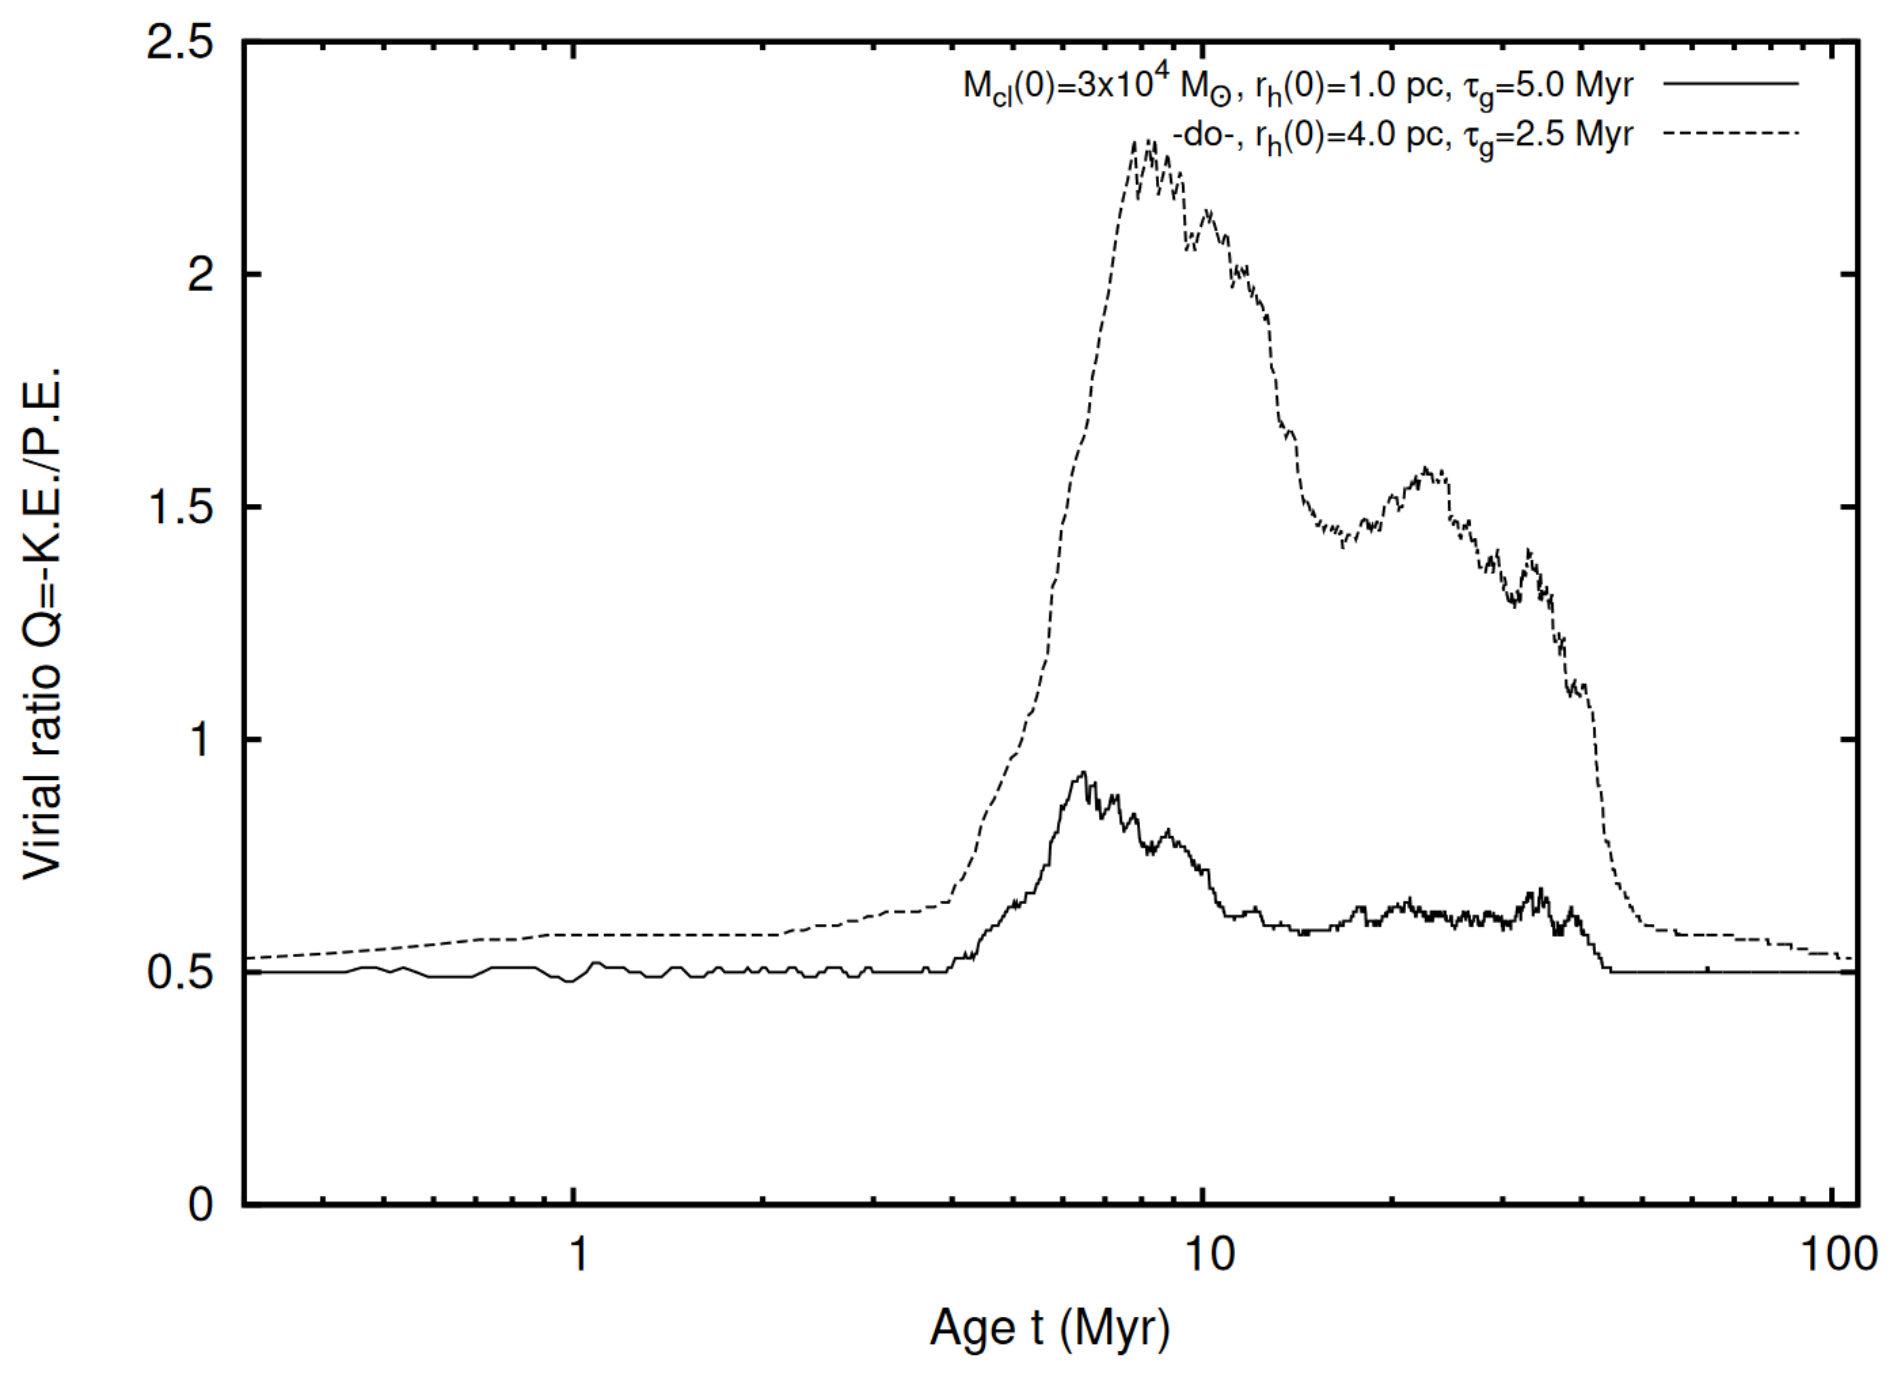
\includegraphics[width=0.8\textwidth]{fig/c1/virialisation_placid_gas_expulsion.png}
	\caption[The evolution of the virial ratio of simulated star clusters with a `placid' model of explosive feedback]{The evolution of the virial ratio of simulated star clusters with a `placid' model of explosive feedback. Simulations were conducted given a cluster of mass  $3\times10^4$~\MSun, with the dashed line showing a cluster with an initial half-mass radius of 1~pc and the solid line showing a cluster with an initial half-mass radius of 4~pc. \emph{Credit}: \cite{banerjee_how_2017}.}
	\label{fig:intro:theory:feedback}
\end{figure}

Once stellar winds expel the initial gas a bound cluster formed from, star clusters in the disk of the Milky Way continue to have a somewhat tumultuous life. Young clusters were typically observed to have sizes larger than those predicted by N-body simulations; it is now believed that other processes must inject energy into early young star clusters in order for them to reach their present-day larger sizes \citep{banerjee_how_2017}.

After initial gas expulsion within the cluster stops additional star formation, star clusters are believed to continue interacting with surrounding gas in their parent GMC for multiple Myr. Stellar winds and feedback from supernovae will continue to disperse the GMC well beyond the radius of the cluster, forming a HII region. This causes a `gravitational feedback' effect, where the massive GMC is blown away and net forces on stars in the cluster also add energy to the system, causing the cluster to be supervirial and undergo a phase of expansion \citep{krause_physics_2020}.

The exact physics of this feedback are still under study, although Fig.~\ref{fig:intro:theory:feedback} taken from \cite{banerjee_how_2017} shows the virial ratio of simulated star clusters with respect to time, for an intermediate or `placid' model of explosive stellar feedback. Within the first 10~Myr of the cluster's lives, feedback causes them to become supervirial. Once the parent GMC has been dispersed, the clusters continue to expand, before eventually reaching dynamical equilibrium and returning to a state with $Q\approx0.5$ after a few tens of Myr. These simulations echo the results of \cite{kuhn_kinematics_2019}, who studied 28 young stellar groups with \gaia\ DR2 and found that 75\% were undergoing expansion (i.e. are supervirial). 

All star clusters are expected to lose a significant portion of their initial mass during this phase of expansion. It has been theorised that bound clusters that form with low initial masses or high initial radii may even be completely destroyed in the initial phase of feedback and expansion, which ought to be visible as unbound cluster remnants \citep{krause_physics_2020}.


\subsubsection{Evaporation and destruction (upto \textasciitilde1~Gyr)}

Since OCs are rarely observed at ages greater than $\sim1$~Gyr, it is clear that some processes eventually destroy them over time. This is believed to happen in three ways.

Firstly, stellar evolution will gradually cause mass loss in a cluster, with more massive stars undergoing supernovae and evolving into compact remnants, losing a significant proportion of their mass in the process. However, since most stars are more compact M, K, or G stars with lifetimes significantly longer than the typical maximum OC lifetime of 1~Gyr, this effect is relatively insignificant during the lifespan of an OC \citep{krause_physics_2020}.

Secondly, clusters gradually lose stars over time in a process known as evaporation. The stars in a cluster will not all have the same velocity; a cluster in dynamical equilibrium will have an isothermal velocity dispersion that is approximately Maxwellian. Some stars with velocities at the tail end of this distribution will have velocities higher than the escape velocity of the cluster $v_\text{esc}$, and will be ejected from the cluster. Over time, two and three-body interactions will accelerate some stars preferentially and ensure that a small proportion of cluster members always have velocities greater than the cluster's $v_\text{esc}$ \citep{portegies_zwart_young_2010,krause_physics_2020}. Stars are preferentially ejected via the cluster's $L_1$ and $L_2$ Lagrange points relative to the tidal field of the Milky Way, which produces the observed tidal tails of many clusters in \gaia\ \citep{portegies_zwart_young_2010,tarricq_structural_2022}. Less commonly, stars will still be ejected in a random direction (opposed to via a Lagrange point), producing an additional spherical `coma' or `corona' of recently ejected stars around a cluster, an effect that has also been observed in \gaia\ data for a number of nearby OCs \citep{meingast_extended_2021,tarricq_structural_2022}.

Finally, star clusters are theorised to be heavily disrupted by tidal `shocks' (perturbations). Reasonably often within every 1~Gyr, star clusters in the Milky Way's disk are expected to come close to or even collide with various pieces of massive galactic structure, such as GMCs or transient spiral arms. The tidal perturbations from these interactions increase the energy of stars in a cluster and should cause considerable mass loss. Due to the rarity of these events, they are yet to be directly observed for OCs in the Milky Way; nevertheless, simple theoretical arguments can show that these events will occur reasonably often for any star cluster in the disk. Especially within the first 1~Gyr of an OC's life, tidal shocks are expected to be a major (and potentially even dominant) method of star cluster destruction \citep{krause_physics_2020}.


% ---------------------------------------
\section{The structure of this thesis}
\label{sec:intro:structure}

The remaining structure of this thesis will be as follows:

\textbf{Chapter \ref{sec:comparison}: \nameref{sec:comparison}} \\[0.2em]
In the first study of this thesis, I compare clustering algorithms for OC retrieval in \gaia\ DR2 data. I review a number of different algorithms, before settling on three for use in the study. I develop methods to use these algorithms in a blind search, including a statistical density test to remove false positive clusters. I then use them to look for 100 OCs in \gaia\ data from the catalogue of \cite{kharchenko_global_2013}, as well as a wider sample of 1385 OCs that were less well studied. A further development of the DBSCAN algorithm, HDBSCAN, was found to be the most effective algorithm for OC retrieval. Additionally, 41 new OCs were detected in the study.

\textbf{Chapter \ref{sec:census}: \nameref{sec:census}} \\[0.2em]
Having refined an initial clustering methodology in Chapter~\ref{sec:comparison}, I conduct the largest ever blind search for OCs in \gaia\ data, using HDBSCAN and data from \gaia\ DR3 down to magnitude $G\sim20$. To further refine the results, I use a Bayesian neural network to derive the probablility of clusters being a single population of stars. In addition, I use a similar Bayesian neural network to derive ages, extinctions, and distances to the clusters in the work. A catalogue of 7167 clusters is produced, 2387 of which are candidate new objects and 4782 of which crossmatch to objects in the literature. 4105 clusters are in a high-quality sample of objects, including 739 of which are new. OC membership lists resulting from this method generally contain more member stars than in previous literature works, and often have tidal tails. It is possible to rule out over 1000 clusters from the pre-\gaia\ catalogue of \cite{kharchenko_global_2013} that I am unable to detect. However, some of the clusters recovered in this chapter appear more compatible with unbound moving groups, and will require further classification with a dynamical methodology.

\textbf{Chapter \ref{sec:dynamics}: \nameref{sec:dynamics}} \\[0.2em]
In the third scientific chapter of this thesis, I develop methodologies to accurate determine whether or not OC candidates in \gaia\ data are gravitationally bound, aiming to determine accurate masses, velocity dispersions, and radii for the clusters in the catalogue from Chapter \ref{sec:census}. 
\todo{add more here once dynamics section is finalised.}

\textbf{Chapter \ref{sec:conclusion}: \nameref{sec:conclusion}} \\[0.2em]

Finally, I present an overview of all the work contained within this thesis. I discuss the contribution of this thesis to the scientific literature. I also discuss the future of OC science in the \gaia\ era and beyond, and  suggest a number of future avenues for research leading on from this thesis.
\todo{make sure this makes sense once conclusion is written}




% Template:
% \textbf{Chapter \ref{sec:intro}} \\[0.2em]
% \blindtext
